% **** Szablon pracy magisterskiej, licencjackiej lub inżynierskiej ****

\documentclass[polish,12pt,twoside,a4paper]{report}

% *************** Definicje stylu dokumentu ***************

% *********************************************************************************
% W pliku tym zdefiniowany jest wygl¹d dokumentu.
% Zmiany tutaj nie s¹ konieczne o ile nie zamierzasz zmieniaæ wygl¹du dokumentu.
% *********************************************************************************

% *************** Za³adowanie pakietów ***************
\usepackage[a4paper,twoside,left=2.0cm,right=1.5cm,top=1.5cm,bottom=1.5cm]{geometry}
\usepackage[T1]{fontenc}
%\usepackage[cp1250]{inputenc}
\usepackage[utf8]{inputenc}
\usepackage[polish]{babel}
\usepackage{amsmath}
\usepackage{amsfonts}
\usepackage{graphicx}
\usepackage{graphics}
\usepackage{times}
\usepackage{indentfirst}%wciecia a nowych akapitach

\usepackage{hyperref}
\usepackage[dvipsnames]{xcolor}
\usepackage{float}
\usepackage{subfigure}
\raggedbottom

\selectlanguage{polish}

%szerokoœœ wciêæ
\setlength{\parindent}{1.25cm}

%numeracja stron
\usepackage{fancyhdr}
\pagestyle{fancy}
\fancyhf{} % usun biezace ustawienia pagin
\fancyhead[LE,RO]{ }
\fancyhead[LO]{ }
\fancyhead[RE]{ }
\fancyfoot[LE,RO]{\small\thepage}
\fancyfoot[LO]{ }
\fancyfoot[RE]{ }
\renewcommand{\headrulewidth}{0.0pt}
\renewcommand{\footrulewidth}{0.0pt}
\addtolength{\headheight}{0.0pt} % pionowy odstep na kreske
\fancypagestyle{plain}{%
\fancyhead{} % usun p. górne na stronach pozbawionych
% numeracji (plain)
\renewcommand{\headrulewidth}{0.0pt} % pozioma kreska
}

% *************** Definicje niektórych kolorów ***************
\usepackage{color}

\definecolor{greenyellow}   {cmyk}{0.15, 0   , 0.69, 0   }
\definecolor{yellow}        {cmyk}{0   , 0   , 1   , 0   }
\definecolor{goldenrod}     {cmyk}{0   , 0.10, 0.84, 0   }
\definecolor{dandelion}     {cmyk}{0   , 0.29, 0.84, 0   }
\definecolor{apricot}       {cmyk}{0   , 0.32, 0.52, 0   }
\definecolor{peach}         {cmyk}{0   , 0.50, 0.70, 0   }
\definecolor{melon}         {cmyk}{0   , 0.46, 0.50, 0   }
\definecolor{yelloworange}  {cmyk}{0   , 0.42, 1   , 0   }
\definecolor{orange}        {cmyk}{0   , 0.61, 0.87, 0   }
\definecolor{burntorange}   {cmyk}{0   , 0.51, 1   , 0   }
\definecolor{bittersweet}   {cmyk}{0   , 0.75, 1   , 0.24}
\definecolor{redorange}     {cmyk}{0   , 0.77, 0.87, 0   }
\definecolor{mahogany}      {cmyk}{0   , 0.85, 0.87, 0.35}
\definecolor{maroon}        {cmyk}{0   , 0.87, 0.68, 0.32}
\definecolor{brickred}      {cmyk}{0   , 0.89, 0.94, 0.28}
\definecolor{red}           {cmyk}{0   , 1   , 1   , 0   }
\definecolor{orangered}     {cmyk}{0   , 1   , 0.50, 0   }
\definecolor{rubinered}     {cmyk}{0   , 1   , 0.13, 0   }
\definecolor{wildstrawberry}{cmyk}{0   , 0.96, 0.39, 0   }
\definecolor{salmon}        {cmyk}{0   , 0.53, 0.38, 0   }
\definecolor{carnationpink} {cmyk}{0   , 0.63, 0   , 0   }
\definecolor{magenta}       {cmyk}{0   , 1   , 0   , 0   }
\definecolor{violetred}     {cmyk}{0   , 0.81, 0   , 0   }
\definecolor{rhodamine}     {cmyk}{0   , 0.82, 0   , 0   }
\definecolor{mulberry}      {cmyk}{0.34, 0.90, 0   , 0.02}
\definecolor{redviolet}     {cmyk}{0.07, 0.90, 0   , 0.34}
\definecolor{fuchsia}       {cmyk}{0.47, 0.91, 0   , 0.08}
\definecolor{lavender}      {cmyk}{0   , 0.48, 0   , 0   }
\definecolor{thistle}       {cmyk}{0.12, 0.59, 0   , 0   }
\definecolor{orchid}        {cmyk}{0.32, 0.64, 0   , 0   }
\definecolor{darkorchid}    {cmyk}{0.40, 0.80, 0.20, 0   }
\definecolor{purple}        {cmyk}{0.45, 0.86, 0   , 0   }
\definecolor{plum}          {cmyk}{0.50, 1   , 0   , 0   }
\definecolor{violet}        {cmyk}{0.79, 0.88, 0   , 0   }
\definecolor{royalpurple}   {cmyk}{0.75, 0.90, 0   , 0   }
\definecolor{blueviolet}    {cmyk}{0.86, 0.91, 0   , 0.04}
\definecolor{periwinkle}    {cmyk}{0.57, 0.55, 0   , 0   }
\definecolor{cadetblue}     {cmyk}{0.62, 0.57, 0.23, 0   }
\definecolor{cornflowerblue}{cmyk}{0.65, 0.13, 0   , 0   }
\definecolor{midnightblue}  {cmyk}{0.98, 0.13, 0   , 0.43}
\definecolor{navyblue}      {cmyk}{0.94, 0.54, 0   , 0   }
\definecolor{royalblue}     {cmyk}{1   , 0.50, 0   , 0   }
\definecolor{blue}          {cmyk}{1   , 1   , 0   , 0   }
\definecolor{cerulean}      {cmyk}{0.94, 0.11, 0   , 0   }
\definecolor{cyan}          {cmyk}{1   , 0   , 0   , 0   }
\definecolor{processblue}   {cmyk}{0.96, 0   , 0   , 0   }
\definecolor{skyblue}       {cmyk}{0.62, 0   , 0.12, 0   }
\definecolor{turquoise}     {cmyk}{0.85, 0   , 0.20, 0   }
\definecolor{tealblue}      {cmyk}{0.86, 0   , 0.34, 0.02}
\definecolor{aquamarine}    {cmyk}{0.82, 0   , 0.30, 0   }
\definecolor{bluegreen}     {cmyk}{0.85, 0   , 0.33, 0   }
\definecolor{emerald}       {cmyk}{1   , 0   , 0.50, 0   }
\definecolor{junglegreen}   {cmyk}{0.99, 0   , 0.52, 0   }
\definecolor{seagreen}      {cmyk}{0.69, 0   , 0.50, 0   }
\definecolor{green}         {cmyk}{1   , 0   , 1   , 0   }
\definecolor{forestgreen}   {cmyk}{0.91, 0   , 0.88, 0.12}
\definecolor{pinegreen}     {cmyk}{0.92, 0   , 0.59, 0.25}
\definecolor{limegreen}     {cmyk}{0.50, 0   , 1   , 0   }
\definecolor{yellowgreen}   {cmyk}{0.44, 0   , 0.74, 0   }
\definecolor{springgreen}   {cmyk}{0.26, 0   , 0.76, 0   }
\definecolor{olivegreen}    {cmyk}{0.64, 0   , 0.95, 0.40}
\definecolor{rawsienna}     {cmyk}{0   , 0.72, 1   , 0.45}
\definecolor{sepia}         {cmyk}{0   , 0.83, 1   , 0.70}
\definecolor{brown}         {cmyk}{0   , 0.81, 1   , 0.60}
\definecolor{tan}           {cmyk}{0.14, 0.42, 0.56, 0   }
\definecolor{gray}          {cmyk}{0   , 0   , 0   , 0.50}
\definecolor{black}         {cmyk}{0   , 0   , 0   , 1   }
\definecolor{white}         {cmyk}{0   , 0   , 0   , 0   } 

% *************** Koniec definicji stylu dokumentu ***************


%definicja przydatnych poleceń
\newcommand{\wydzial}{KOLEGIUM INFORMATYKI STOSOWANEJ}
\newcommand{\kierunek}{Kierunek: INFORMATYKA}
\newcommand{\specjalnosc}{Specjalność: PROGRAMOWANIE}
\newcommand{\autor}{Oleksandr Lobchenko}
\newcommand{\album}{Nr albumu studenta w68317}
\newcommand{\temat}{APLIKACJA DESKTOPOWA "SZPITAL+"}
\newcommand{\prowadzacy}{mgr inż. Ewa Żesławska}
\newcommand{\typpracy}{Praca projektowa programowanie obiektowe C\#}
\newcommand{\miasto}{Rzeszów}
\newcommand{\rok}{2024}

\begin{document}

% *************** Włączenie definicji pierwszych stron ***************
% *************** Strony tytułowe ***************

% ************************************************************
% W tym miejscu znajduje sie definicja wyglądu pierwszych stron:
% strony tytułowej, strony z oświadczeniem o treści pracy
% i strony ze spisem treści
% ************************************************************
% *************** Strona tytułowa ***************
%umieszczenie logo i nazwy uczelni
\noindent
\parbox{65mm}{
\includegraphics[width=13.0cm, height=3.0cm]{logoWSIiZ}}

\vspace{10mm}
\begin{center}
{\Large{}\textbf{\wydzial}}
\end{center}
\vspace{10mm}
\noindent
\hspace{30mm}{\Large{}\textbf{\kierunek}}\\

\noindent
\hspace{30mm}{\Large{}\textbf{\specjalnosc}}
\vspace{30mm}
\begin{center}
	{\large{}\autor}\\
	{\large{}\album}\\
	\vspace{15pt}
	{\huge{}\textbf{\textit{\temat}}}\\
        \vspace{20pt}
	{\normalsize{}Prowadzący: \prowadzacy}\\
	\vspace{100pt}
	{\LARGE{}\textbf{\typpracy}}\\
	\vspace{190pt}
	{\large{}\textbf{\miasto {} \rok}}
\end{center}

% pusta zawartość stopki - brak numeru strony
\thispagestyle{empty}

% *************** Strona z oświadczeniem o treści pracy ***************
\newpage
\text{}

\thispagestyle{empty}
\newpage


% *************** Spis treści ***************
\tableofcontents
% pusta zawartość stopki - brak numeru strony
\thispagestyle{empty}
\newpage

% *************** Koniec pliku front.tex ***************



% *************** Część główna pracy ***************
\chapter*{Wstęp}

\textquotedbl Aplikacja desktopowa Szpital+\textquotedbl{} jest aplikacją mającą na celu zmodernizowanie i usprawnienie codziennych operacji w placówkach medycznych. Jest to program umożliwiający do przechowywania i dodawania informacji dotyczących szpitalu. Medycyna zajmuje bardzo ważną część naszego życia. Dlatego uważam, że ułatwienie komunikacji między pracownikami zaoszczędzi czas i ulepszy jakość pracy.
\addcontentsline{toc}{chapter}{Wstęp}
\newpage
% ********** Rozdział 1 **********
\chapter{Opis założeń projektu}
\section{Cele projetu}
%\subsection{Tytuł pierwszego podpunktu}

Celem głównym projektu jest stworzenie kompleksowej aplikacji desktopowej, mającej na celu usprawnienie procesów zarządzania w środowisku szpitalnym. Aplikacja \textquotedbl Szpital+\textquotedbl{} ma usprawnić gromadzenie danych medycznych oraz zwiększyć efektywność komunikacji w placówce medycznej. Aplikacja posiada 4 klienta, funkcjonalność których się różni:
\renewcommand{\labelenumi}{\alph{enumi})}
\begin{enumerate}
    \item{Klient Głównego Kierownika}
    \item{Klient Kierownika Działu} 
    \item{Klient Recepcjonisty}
    \item{Klient Lekarza}
\end{enumerate}

\section{Wymagania funkcjonalne}

\begin{itemize}
    \item Logowanie do systemu.
    \item Przegląd informacji o siebie lub innym pracowniku.
    \item Możliwość dodawać, usuwać lub zmieniać wizyty.
    \item Możliwość dodawać lub zwalniać pracowników.
    \item Możliwość wylogowania.
    \item Dodanie lub usuwanie zapisów w książkach pacjentów.
    \item Dodanie i usunięcie pacjentów.
\end{itemize}

\section{Wymagania niefunkcjonalne}

\begin{itemize}
    \item \textbf{Łatwy w użyciu i przejrzysty interfejs użytkownika:} interfejs musi odpowiadać nowoczesnym stylom budowania aplikacji GUI.
    \item \textbf{Walidacja danych:} program musi sprawdzać poprawność wpisanych przez użytkownika danych.
    \item \textbf{Wyświetlenie komunikatów:} przy wpisaniu błędnych danych aplikacja ma powiadomić użytkownika o pojawiającym się błędzie.
    \item \textbf{Prawidłowo działająca baza danych:} baza danych ma pozwalać na operacje CRUD i być logicznie zdefiniowana.
\end{itemize}

% ********** Koniec rozdziału **********

\newpage
% ********** Rozdział 2 **********
\chapter{Opis struktury projektu}

Projekt składa się z kilku części: Klasy główne(Models), Klasy używane do nawigacji, Komendy, Klasa do przechowywania ViewModels(NavigateStore) i Klasa do wykorzystania bazy danych. Klasy główne używane są do przechowywania danych z bazy(np. Pracownik lub Wizyta). Klasy nawigacyjne używane są do przechowywania danych i operacji nad danymi pobranych od użytkownika w widoku(View) lub z bazy danych(np. UserInfoViewModel przechowuje informacje pobraną z bazy danych i przenosi ją do UserInfoView). Komendy wykorzystane są do nawigacji, przesłania danych do bazy danych lub otrzymania danych.

\section{Diagram klas}

\begin{figure}[H]
\begin{center}
    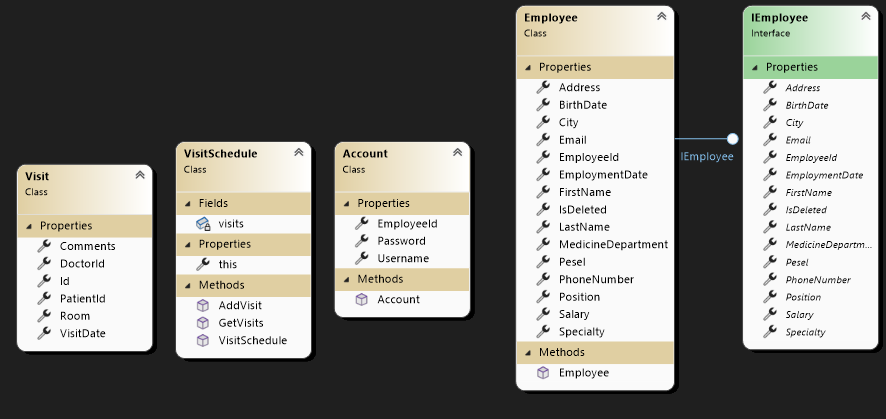
\includegraphics[height=8cm]{images/diag_gl_kl.png}
    \caption{Klasy główne}
\end{center}
\end{figure}

\begin{figure}[H]
\begin{center}
    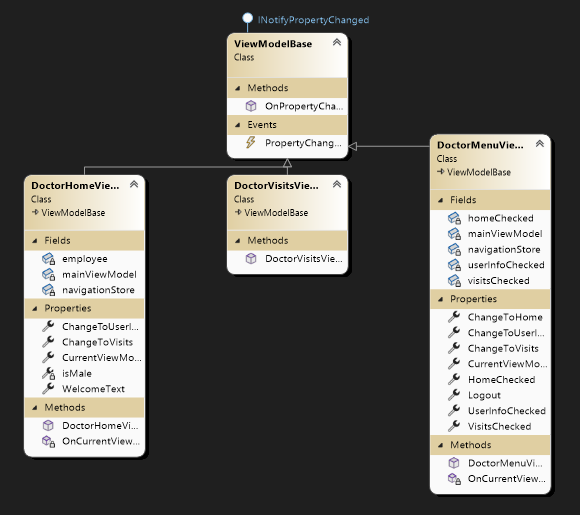
\includegraphics[height=10cm]{images/diag_kl_nav_dok.png}
    \caption{Klasy nawigacyjne dla doktora}
\end{center}
\end{figure}

\begin{figure}[H]
\begin{center}
    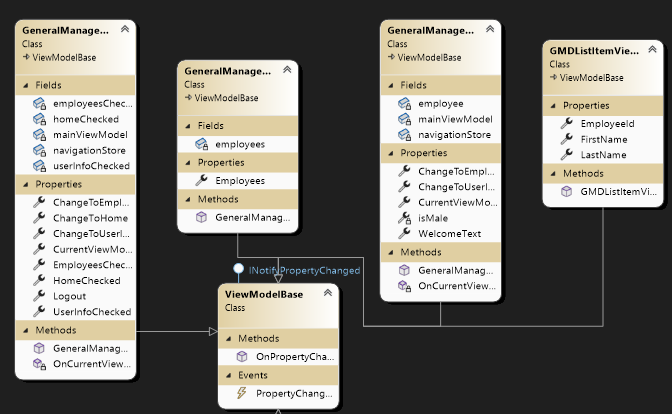
\includegraphics[height=10cm]{images/diag_kl_nav_gen_man.png}
    \caption{Klasy nawigacyjne dla głównego kierownika}
\end{center}
\end{figure}

\begin{figure}[H]
\begin{center}
    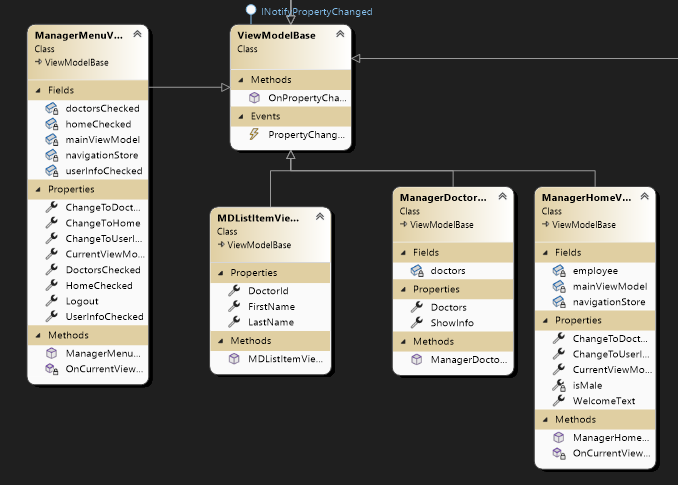
\includegraphics[height=10cm]{images/diag_kl_nav_mang.png}
    \caption{Klasy nawigacyjne dla kierownika}
\end{center}
\end{figure}

\begin{figure}[H]
\begin{center}
    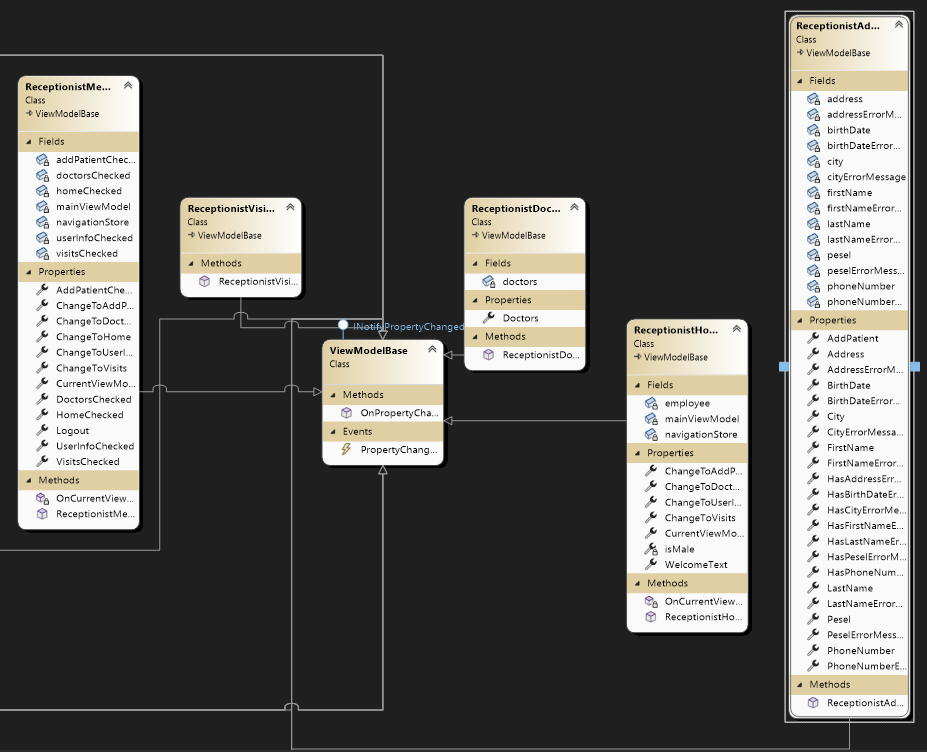
\includegraphics[height=10cm]{images/diag_kl_nav_recep.png}
    \caption{Klasy nawigacyjne dla recepcjonisty}
\end{center}
\end{figure}

\begin{figure}[H]
\begin{center}
    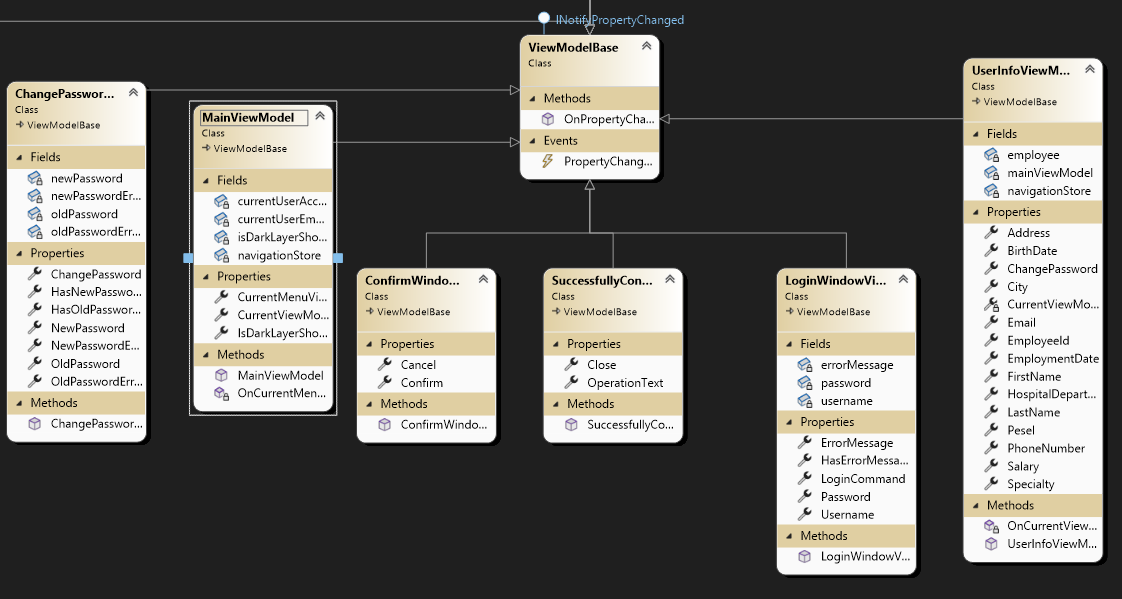
\includegraphics[height=9cm]{images/diag_kl_nav_wszt.png}
    \caption{Klasy nawigacyjne wspólne dla wszystkich klientów}
\end{center}
\end{figure}

\begin{figure}[H]
\begin{center}
    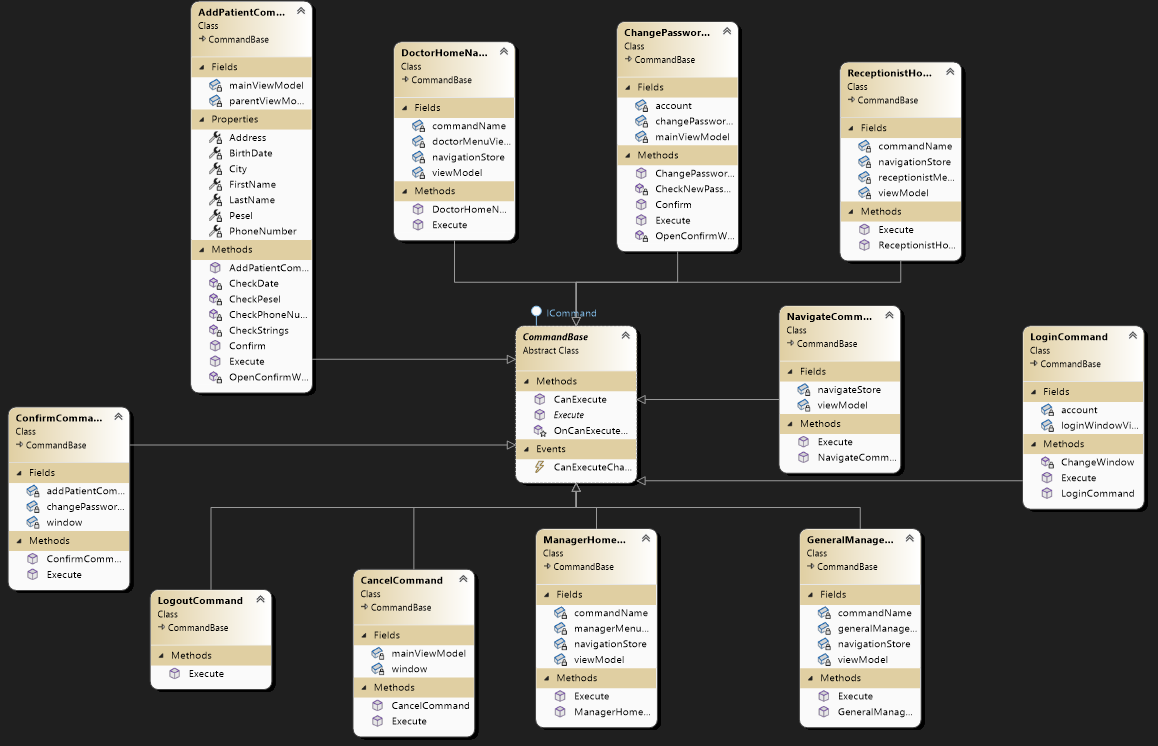
\includegraphics[height=10cm]{images/diag_kl_kom.png}
    \caption{Klasy komend}
\end{center}
\end{figure}

\begin{figure}[H]
\begin{center}
    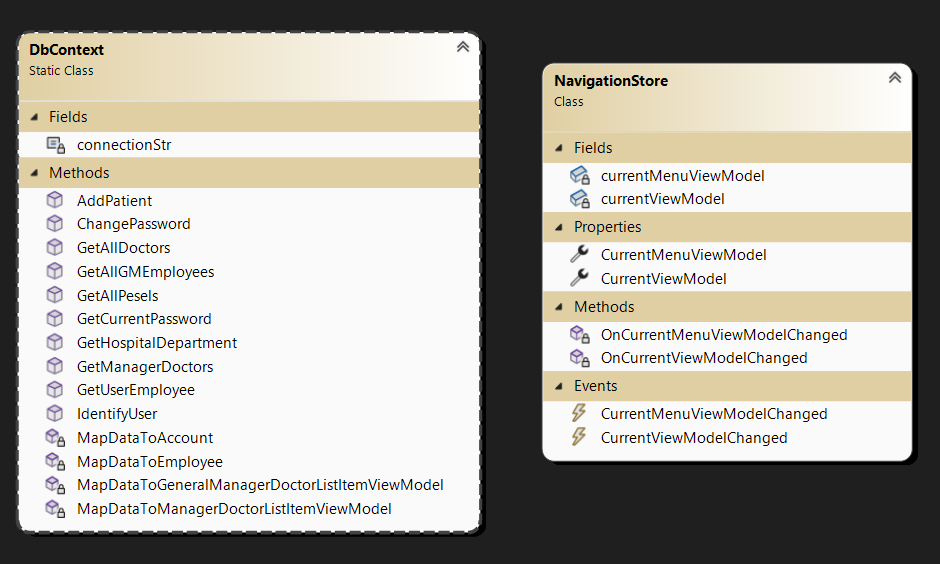
\includegraphics[height=8cm]{images/diag_kl_db_nav.png}
    \caption{Klasy dla bazy danych i przechowywania nawigacji}
\end{center}
\end{figure}

\section{Narzędzie}

Do tworzenia aplikacji \textquotedbl Szpital+\textquotedbl{} korzystałem z narzędzi {\color{blue}\href{https://pl.wikipedia.org/wiki/Windows_Presentation_Foundation}{WPF(Windows Presentation Foundation)}}. Jest to narzędznie do trowrzenia aplikacji desktopowych dla systemów Windows na bazie {\color{blue}\href{https://pl.wikipedia.org/wiki/.NET_Framework}{.Net Framework}}. Wykorzystywuje język opisy interfejsu użytkownika({\color{blue}\href{https://pl.wikipedia.org/wiki/Extensible_Application_Markup_Language}{XAML}}\label{href:XAML}) oraz język programowania {\color{blue}\href{https://pl.wikipedia.org/wiki/C_Sharp}{C\#}}\label{href:c_sh} do implementacji funkcjonalności elementów i innych funckji backend. 

Dodatkowo przestrzegałem {\color{blue}\href{https://en.wikipedia.org/wiki/Model%E2%80%93view%E2%80%93viewmodel}{wzóru architektonicznego MVVM}}(Model-View-ViewModel)\label{href:MVVM}. Jest to wzór który rozdziela graficzny interfejs użytkownika GUI(View) od implementacji logiki biznesowej oraz logiki backend. Związkiem między tymi warstami jest konwerter wartości (ViewModel), który przyjmuje publiczne właściwości modeli(Models) i przekazuje ich do widoków(Views) za pomocą wiązania (Binding).

Do pisania kodu korzystałem z środowiska programistycznego {\color{blue}\href{https://pl.wikipedia.org/wiki/Microsoft_Visual_Studio}{Microsoft Visual Studio}\label{href:VStudio}}.

Także wykorzystełem wtyczki \textquotedbl {\color{blue} \href{https://github.com/charri/Font-Awesome-WPF}{FontAwesome.WPF}}\textquotedbl{} dla dodania ikon jako tekstu dla nawigacji bocznej i wtyczki \textquotedbl {\color{blue}\href{https://github.com/dotnet/corefx}{System.Data.SqlClient}}\textquotedbl{} dla połączenia z bazą danych SQL.

\newpage

\section{Baza danych}

Do stworzenia i zarządzania bazą danych wykorzystywałem {\color{blue}\href{https://en.wikipedia.org/wiki/SQL_Server_Management_Studio}{Microsoft SQL Server Management Studio}}. Na lokalnym serwerze stworzyłem bazę danych "Spzital". Także uzupełniłem bazę losowymi wartościami i dodałem kilka ograniczeń. Na przykład ograniczenie na wprowadzenie do nr\_gabinetu w wizycie większego od 127.

\begin{figure}[H]
\begin{center}
    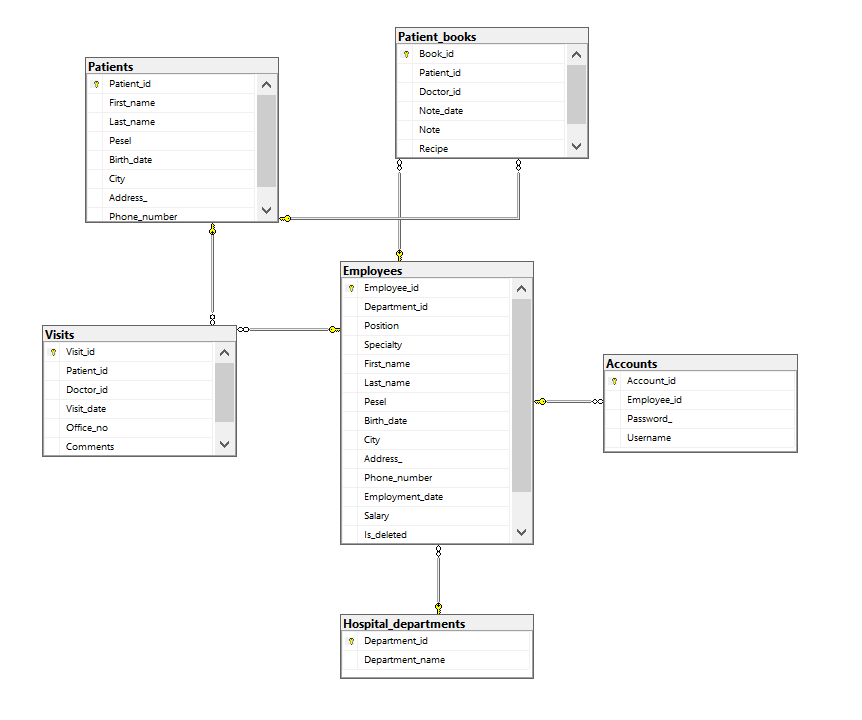
\includegraphics[height=12cm]{images/db_diagram.png}
    \caption{Diagram bazy danych}
\end{center}
\end{figure}

Do pobrania danych z bazy do aplikacji wykorzystuję klasy statycznej DbContext w której są metody robiące zapytania na bazę danych i wracające wartości pobrane z bazy.

\begin{figure}[H]
    \centering
    \subfigure{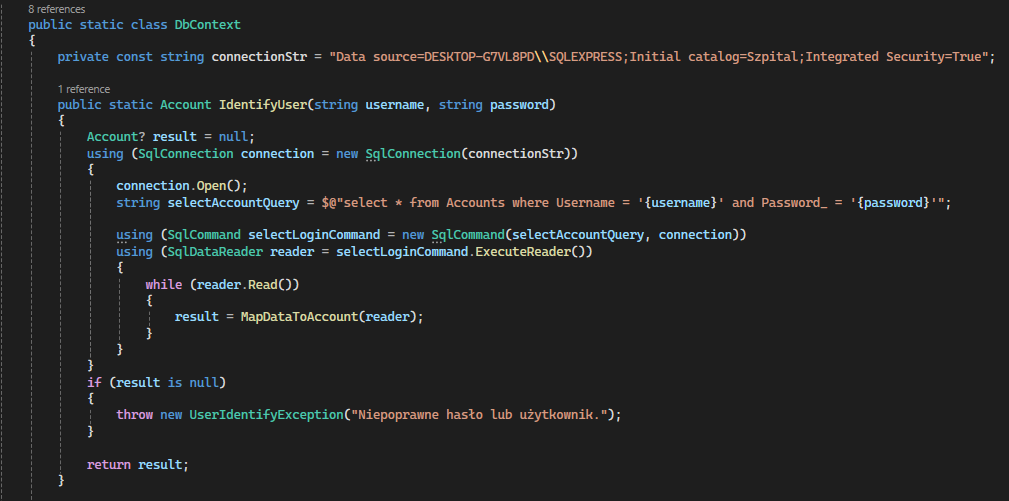
\includegraphics[width=0.7\textwidth]{images/db_cont_klas1.png}} 
    \subfigure{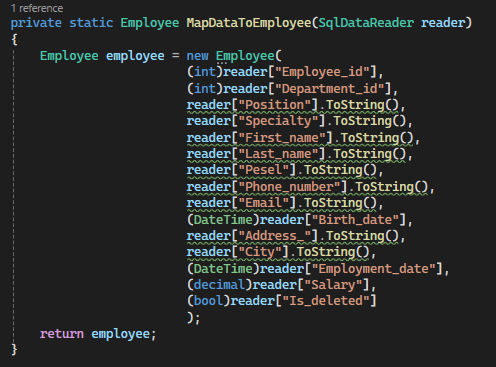
\includegraphics[width=0.7\textwidth]{images/db_cont_klas2.png}} 
    \caption{Klasa do zarządzania bazą danych(Przykładowa metoda)}
\end{figure}

\section{Minimalne wymagania sprzętowe}
\begin{itemize}
    \item System operacyjny: Microsoft Windows 10 lub wyżej
    \item Procesor: x86 lub x64 z szybkością > 800 MHz
    \item RAM: 512 MB
    \item Miejsca na dysku: 25 MB
    \item Zainstalowany .Net 8.0
\end{itemize}


% ********** Koniec rozdziału **********

\newpage
% ********** Rozdział 4 **********
\chapter{Harmonogram realizacji projektu}

\label{sec:harmon_proj}
\section{Diagram Gantta}

\begin{figure}[H]
    \begin{center}
	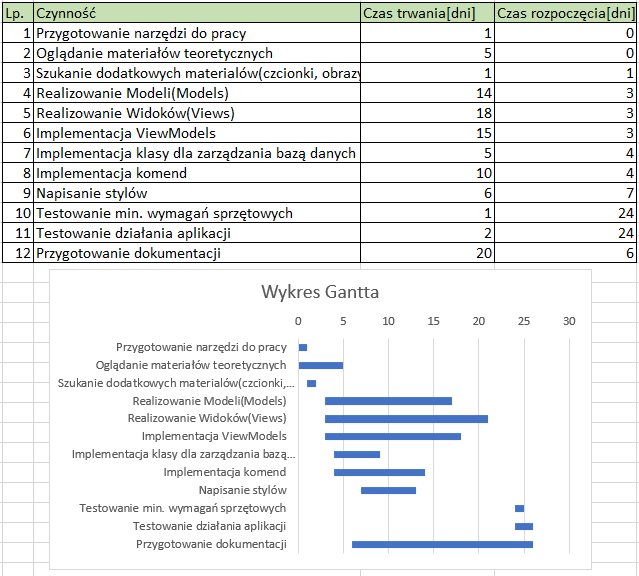
\includegraphics[height=10cm]{images/Wykres_Gantta.png}
        \caption{Wykres Gantta}
    \end{center}
\end{figure}

Zacząłem pracę nad projektem z przygotowania narzędzi do pracy(ustawienia Visual Studio) i oglądania materiałów teoretycznych. Bardzo mi pomogły serie filmików na temat "Architektura MVVM w WPF" na YouTube({\color{blue}\href{https://youtu.be/fZxZswmC_BY?si=Fs_RE23INJFVoy1r}{link}}). Następnie próbowałem zrobić swoją aplikacje na bazie otrzymanej teorii. 

W końcu pozostało mi przetestować minimalne wymagania sprzętowe za pomocą wirtualnej maszyny.


\section{Repozytorium}
Do kontroli wersji oraz przechowywania wykorzystałem systemu Git oraz serwisu internetowego GitHub. Wszystkie pliki źródłowe projektu oraz dokumentacji są umieszczone w tym linku - {\color{blue}\href{https://github.com/clowd1e/Szpital}{Repozytorium GitHub}}.

% ********** Koniec rozdziału **********
\newpage
% ********** Rozdział 4 **********
\chapter{Prezentacja warstwy użytkowej projektu}

\section{Logowanie}

Uruchamiając aplikację, użytkowniku wyświetla się okno logowania:

\begin{figure}[H]
\begin{center}
    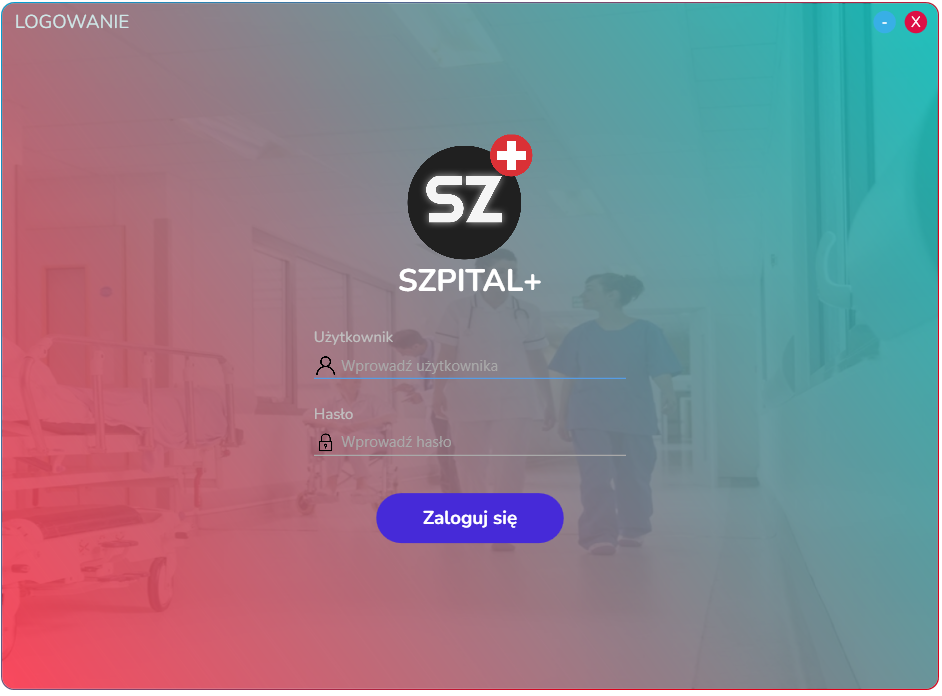
\includegraphics[height=10cm]{images/log_widok.png}
    \caption{Okno logowania}
\end{center}
\end{figure}

W tym oknie został przerobiony górny standardowy panel aplikacji windows. Rozmiar okna 750x550px. Także tło oraz granica zrobione z gradientu. Okno jest trochę zaokrąglone. Po wprowadzeniu danych i naciśnięciu przycisku \textquotedbl Zaloguj się\textquotedbl{} klasa statyczna DbContext sprawdza czy użytkownik istnieje i czy hasło jest poprawne za pomocą polecenia SQL. W przypadku gdy użytkownik poda błędne dane DbContext rzuca wyjątek \textquotedbl UserIdentifyException\textquotedbl{} który jest łapany w LoginCommand, skąd wypisuje się komunikat.

\begin{figure}[H]
\begin{center}
    
\includegraphics[height=10cm]{images/niep_uzyt.png}
    \caption{Wprowadzenie błędnych danych do logowania}
\end{center}
\end{figure}

Jeśli użytkownik istnieje i hasło jest poprawne —logujemy się do aplikacji.

\begin{figure}[H]
    \centering
    \subfigure{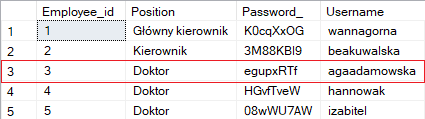
\includegraphics[width=0.6\textwidth]{images/istn_uzyt.png}} 
    \subfigure{
\includegraphics[width=0.3\textwidth]{images/rand_uzyt1.png}}
    \subfigure{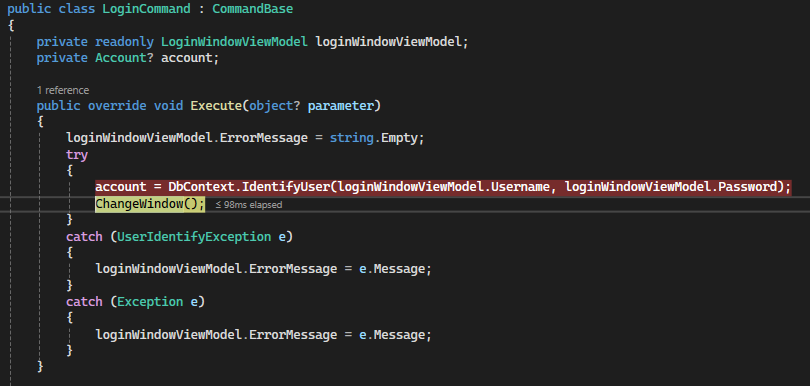
\includegraphics[width=0.8\textwidth]{images/log_kom_exe.png}}
    \caption{Logowanie (DbContext nie rzucił wyjątku)}
\end{figure}

\section{Główne okno}

MainWindow(Okno główne) składa się z trzech części:

\begin{figure}[H]
\begin{center}
    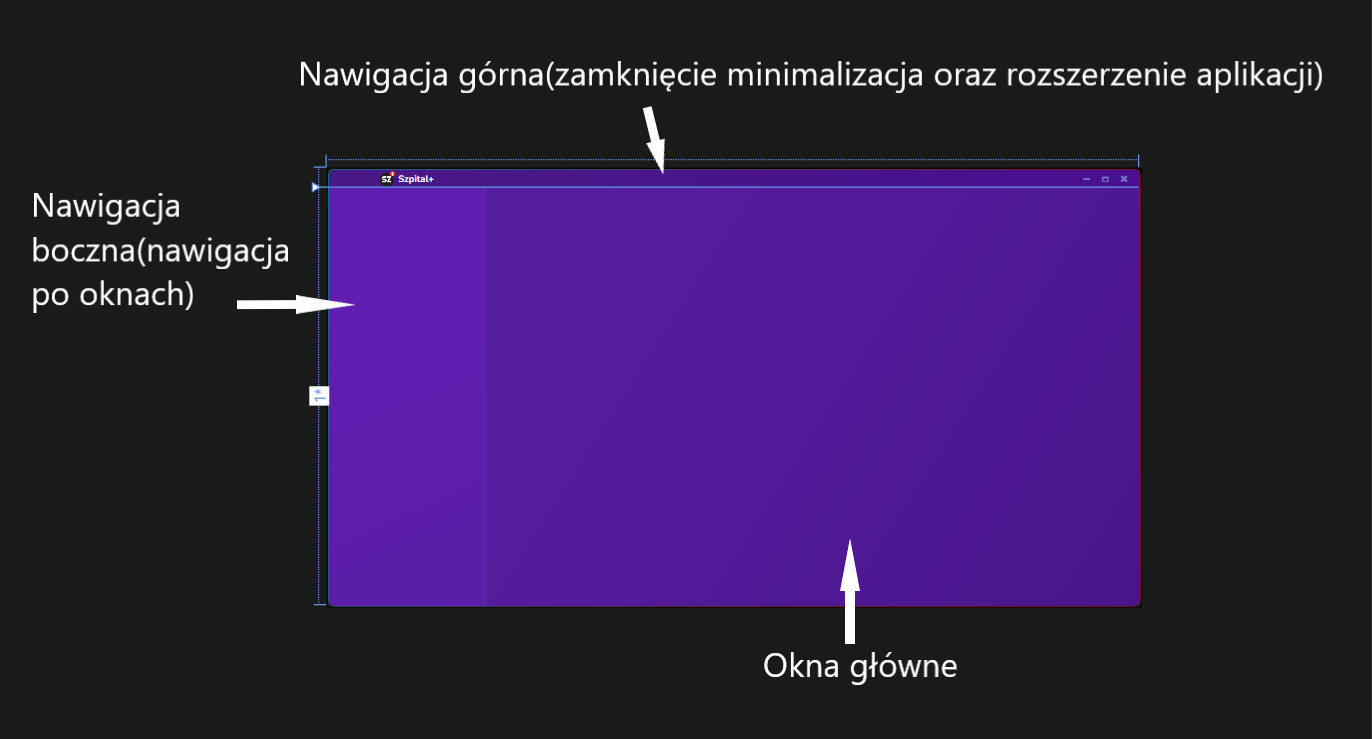
\includegraphics[height=8cm]{images/mainwindow.png}
    \caption{Główne okno}
\end{center}
\end{figure}

Aplikacja pobiera dane z bazy i ze względu na to, na jakim stanowisku pracuje użytkownik, wykorzystuje jeden z szablonów dotyczący jego posady żeby stworzyć nowy wygląd nawigacji bocznej.

\begin{figure}[H]
\begin{center}
    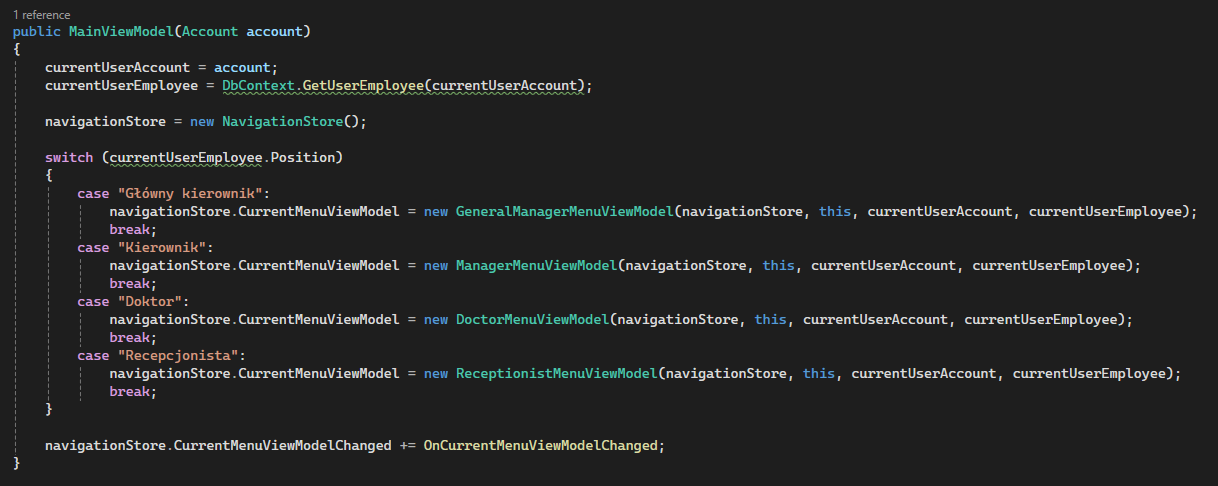
\includegraphics[height=7cm]{images/mainviewmodel_const.png}
    \caption{Pobieranie stanowiska użytkownika i przypisanie nowego wyglądu}
\end{center}
\end{figure}

Na przykład do aplikacji został zalogowany Recepcjonista.
Wtedy wygląd jego aplikacji będzie następny(także aplikacja sprawdza jaki zwrot wykorzystać na pulpicie ze względu na płeć osoby):

\begin{figure}[H]
\begin{center}
    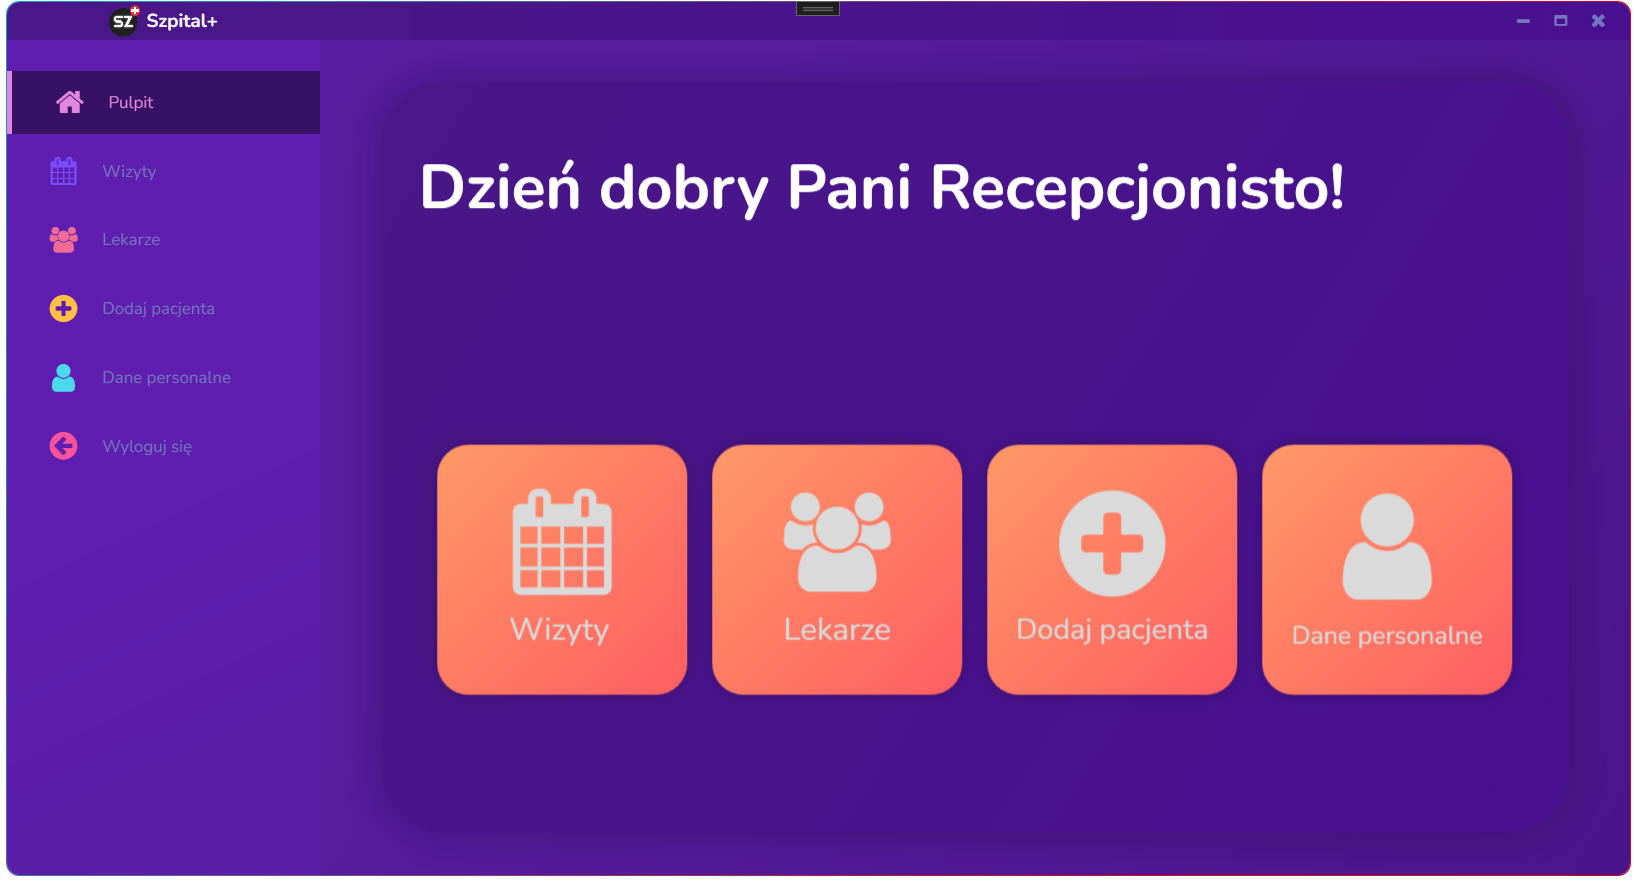
\includegraphics[height=8cm]{images/recep_view.png}
    \caption{Wygląd aplikacji recepcjonisty(Katarzyna Pabiniak)}
\end{center}
\end{figure}

\begin{figure}[H]
\begin{center}
    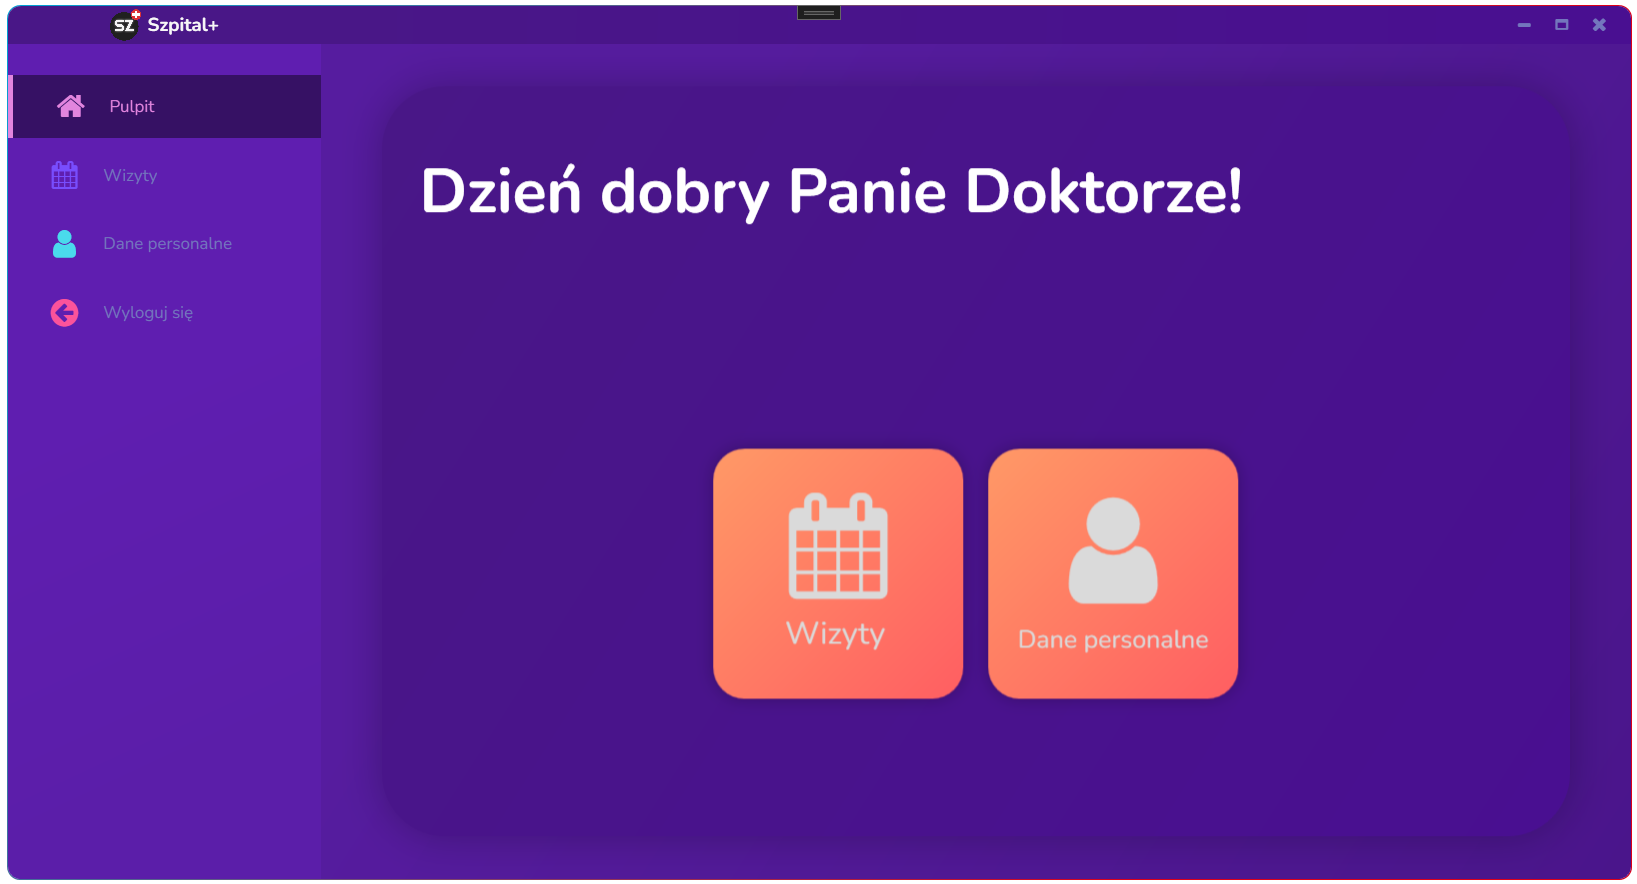
\includegraphics[height=8cm]{images/doktor_view.png}
    \caption{Wygląd aplikacji doktora(Filip Jabcoń)}
\end{center}
\end{figure}

Każdy klient na panelu nawigacyjnym bocznym ma przyciski: pulpit(okno z nawigacją), dane personalne(dane o użytkowniku), wyloguj się(wylogowanie z systemu i wracanie do okna logowania).

\section{Dane personalne}

\begin{figure}[H]
    \centering
    \subfigure{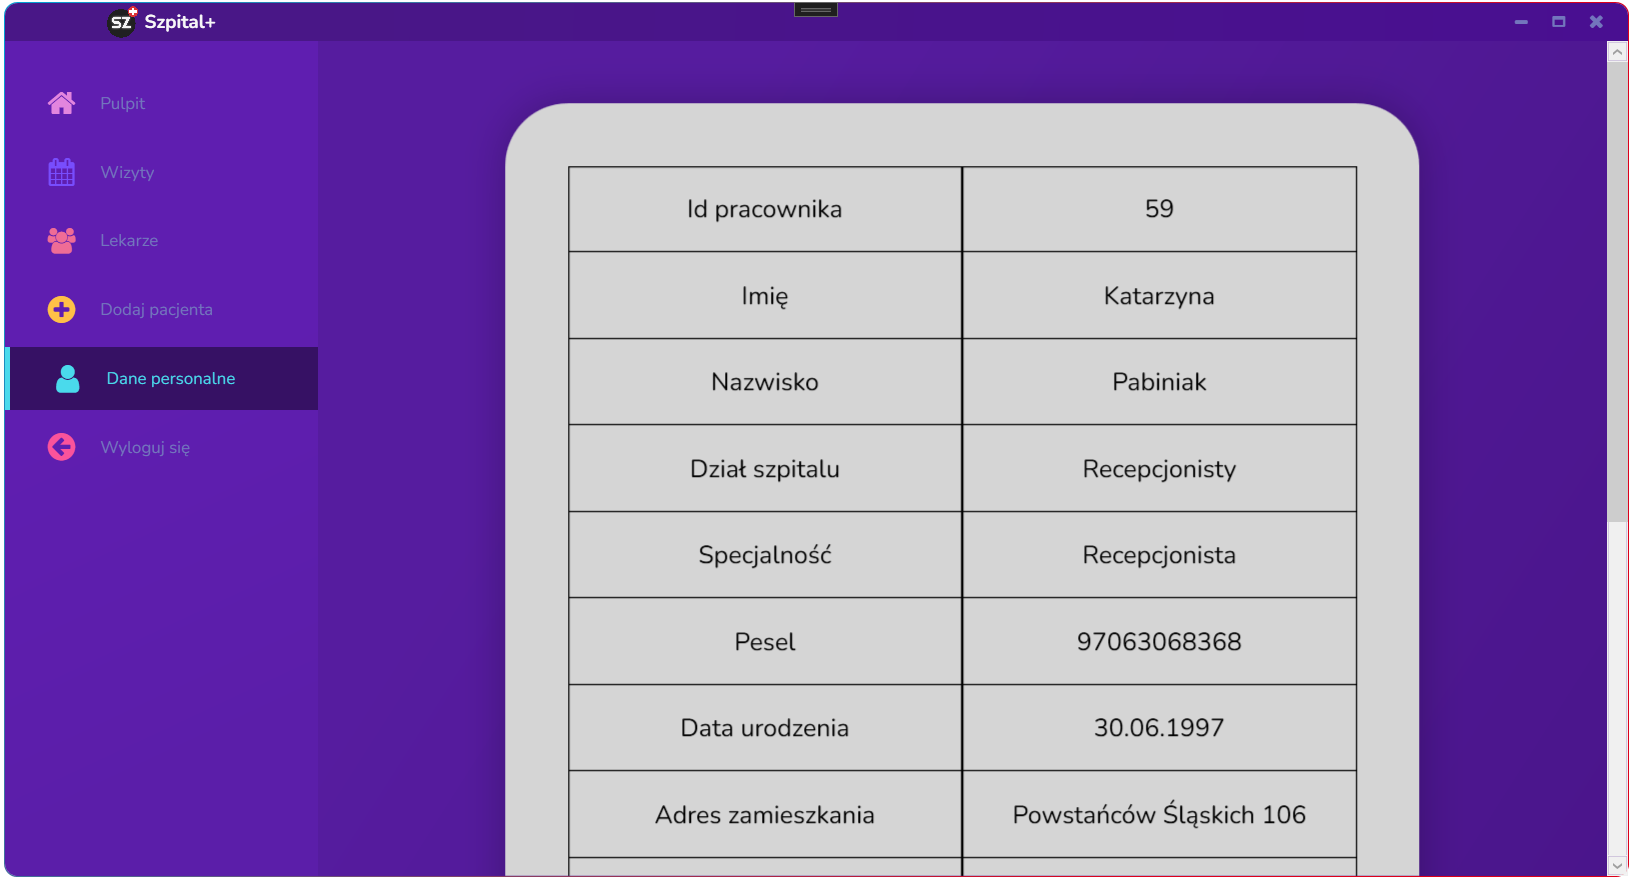
\includegraphics[width=0.7\textwidth]{images/dane_person1.png}} 
    \subfigure{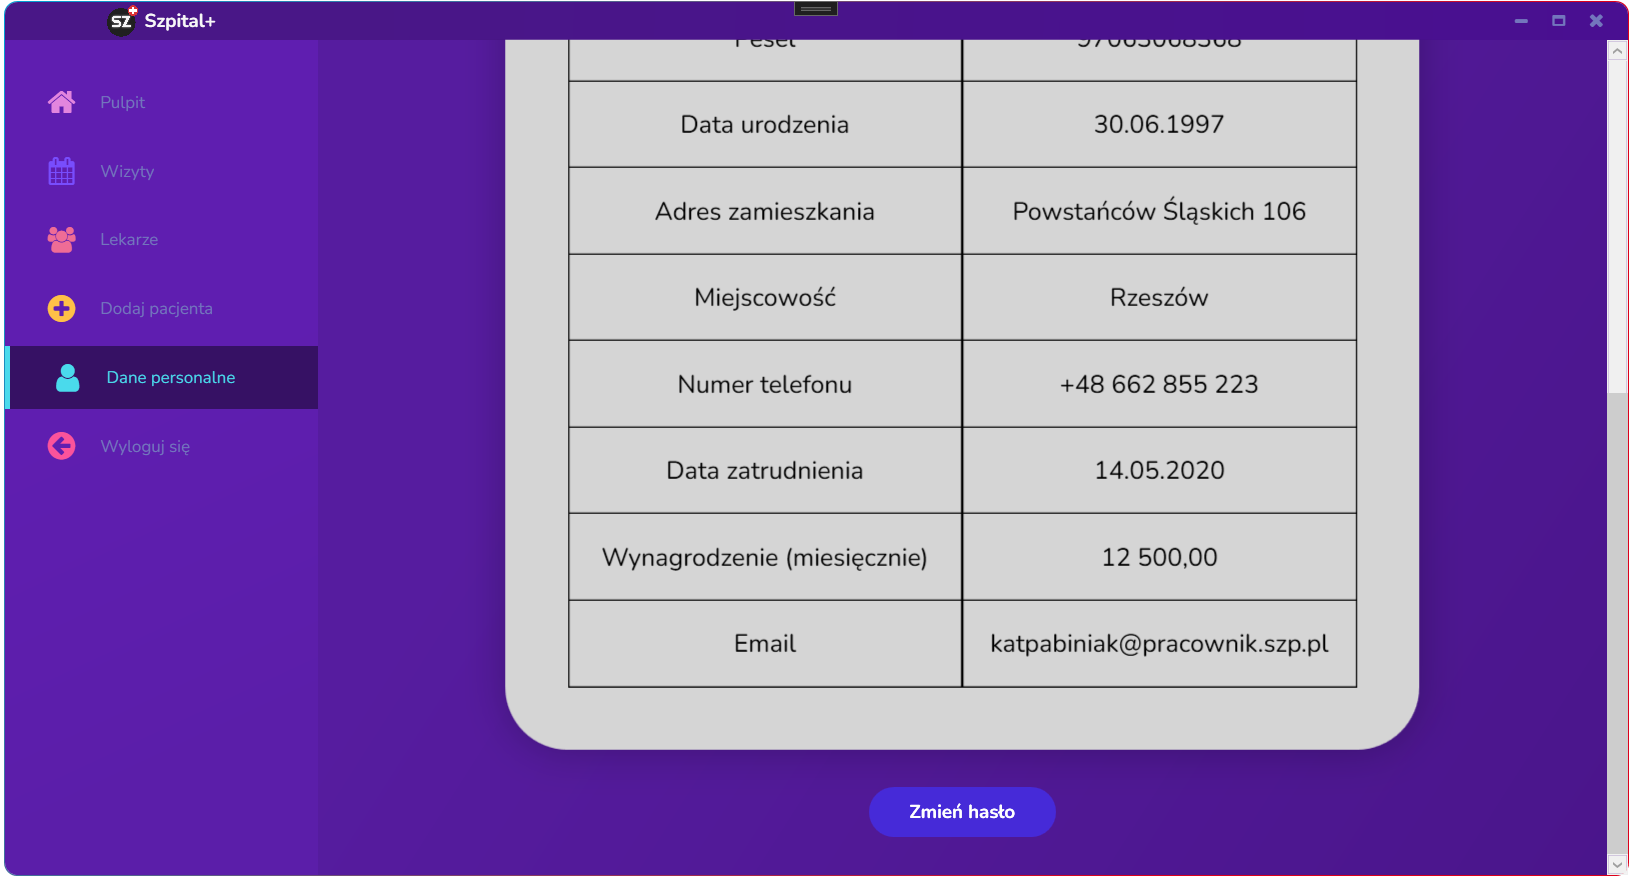
\includegraphics[width=0.7\textwidth]{images/dane_person2.png}}
\caption{Wygląd danych personalnych}
\end{figure}

\section{Zmienianie hasła}

Zmienianie hasła dostępne na dołu okna Dane personalne za pomocą przycisku.

\begin{figure}[H]
\begin{center}
    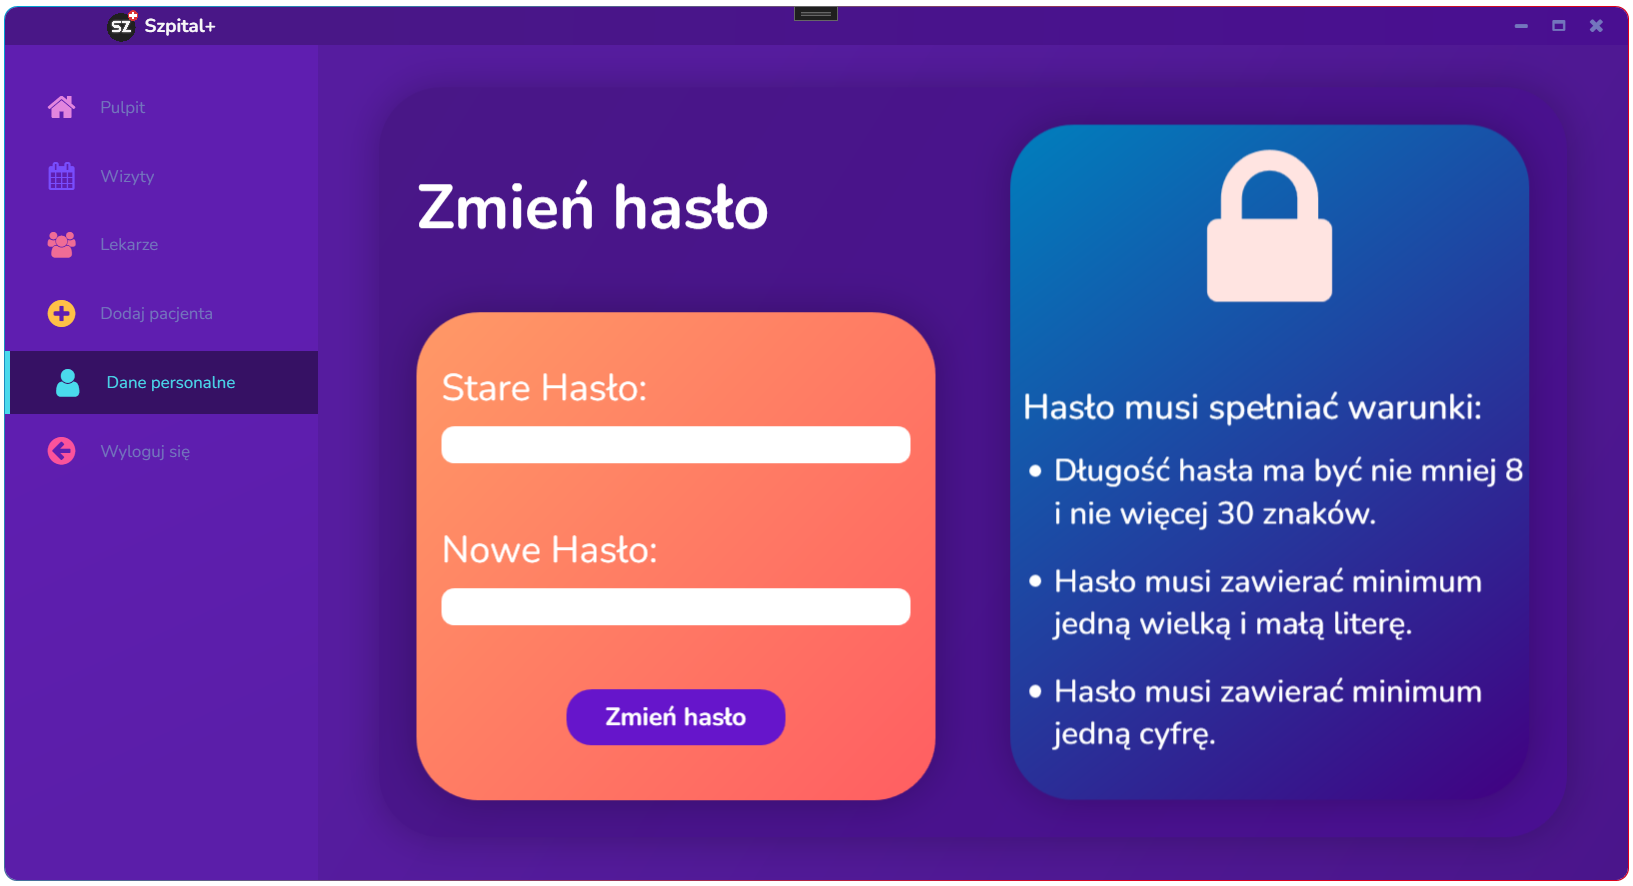
\includegraphics[height=6cm]{images/zmien_hasl.png}
    \caption{Wygląd okna \textquotedbl Zmień hasło\textquotedbl{}}
\end{center}
\end{figure}

Jeśli stare hasło nie będzie takim samym jak w bazie danych wystąpi błąd:

\begin{figure}[H]
\begin{center}
    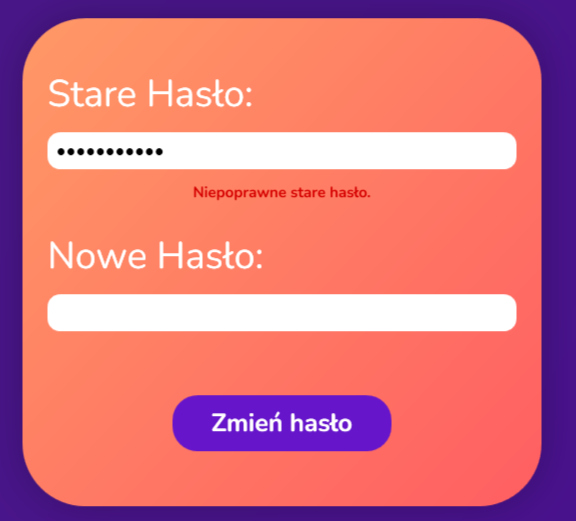
\includegraphics[height=5cm]{images/niepop_stare_hasl.png}
    \caption{Błąd przy wpisaniu starego hasła}
\end{center}
\end{figure}

\section{Sprawdzenie nowego hasła}
Sprawdzenie nowego hasła odbywa się za pomocą {\color{blue}\href{https://en.wikipedia.org/wiki/Regular_expression}{wyrażenia regularnego}}({\color{blue}\href{https://learn.microsoft.com/en-us/dotnet/standard/base-types/regular-expression-language-quick-reference}{Klasa Regex}}).

\begin{figure}[H]
\begin{center}
    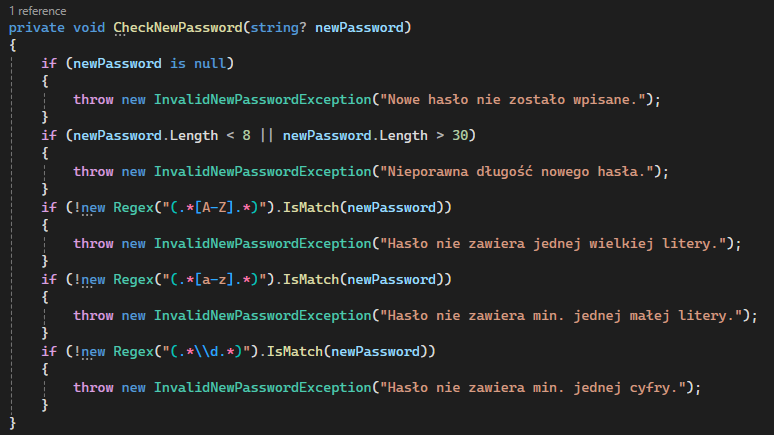
\includegraphics[height=7cm]{images/sprawdz_hasl.png}
    \caption{Metoda do sprawdzenia nowego hasła}
\end{center}
\end{figure}

\begin{figure}[H]
\begin{center}
    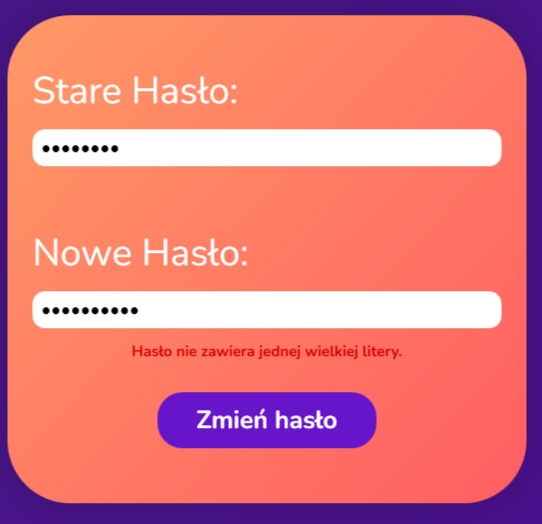
\includegraphics[height=6cm]{images/blad_nowe_hasl.png}
    \caption{Wystąpienie błędu przy nowym hasłu}
\end{center}
\end{figure}

Jeśli nowe hasło odpowiada wszystkim warunkom, pojawia się okno do zatwierdzenia operacji. Przy tym interakcja z głownem oknem jest niemożliwa dopóki użykownik anuluje lub zatwierdzi operację.

\begin{figure}[H]
\begin{center}
    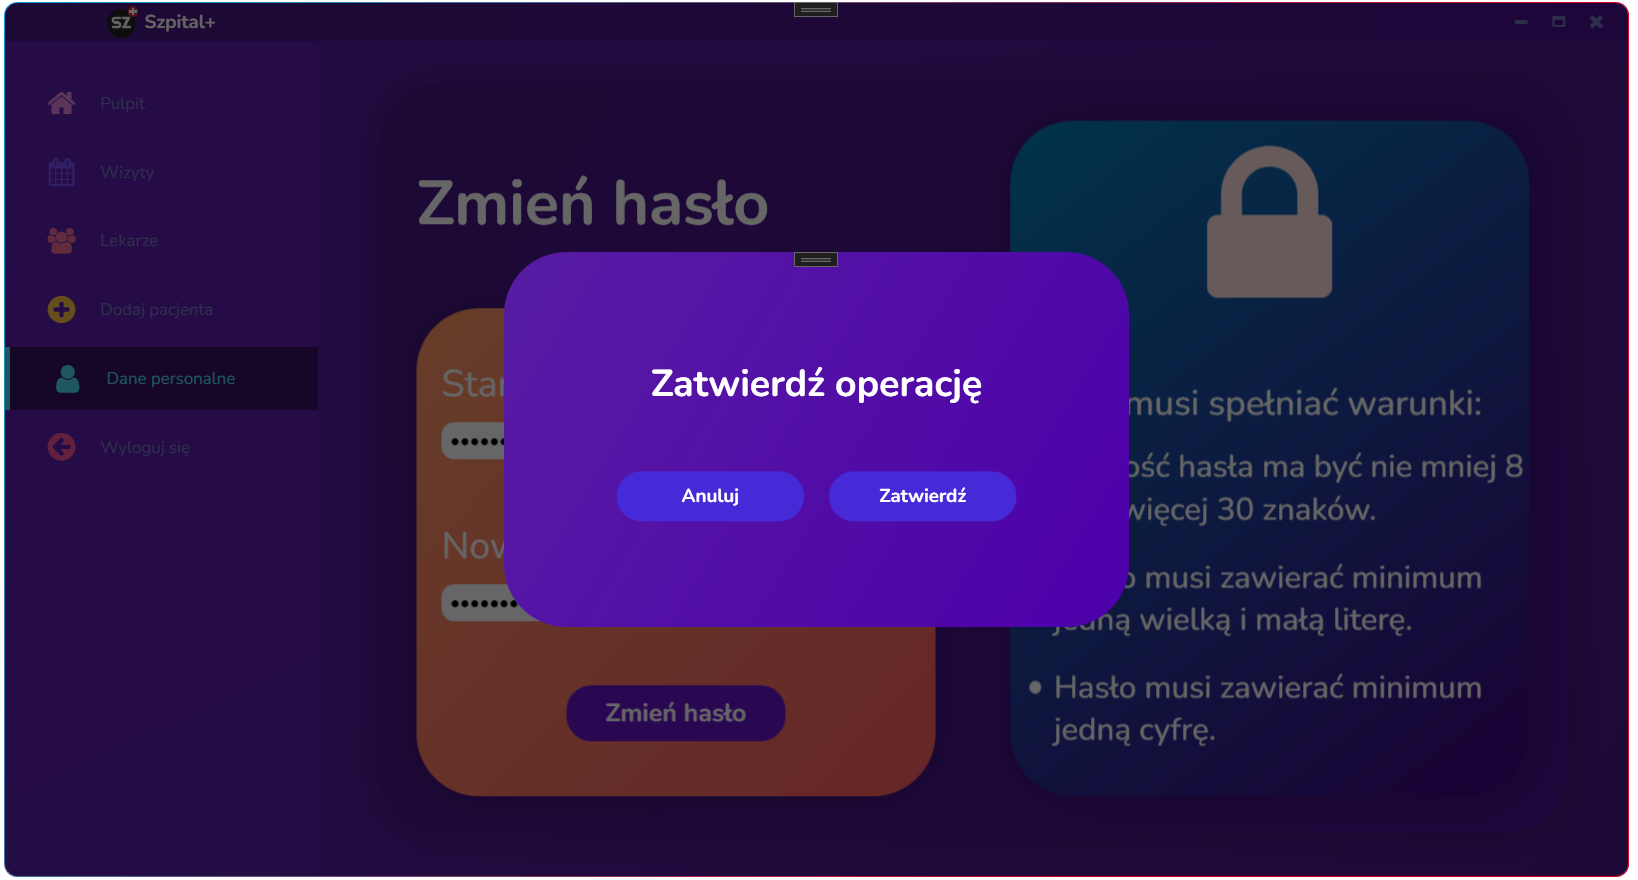
\includegraphics[height=8cm]{images/zatw_oper.png}
    \caption{Okno do zatwierdzenia operacji}
\end{center}
\end{figure}

\begin{figure}[H]
\begin{center}
    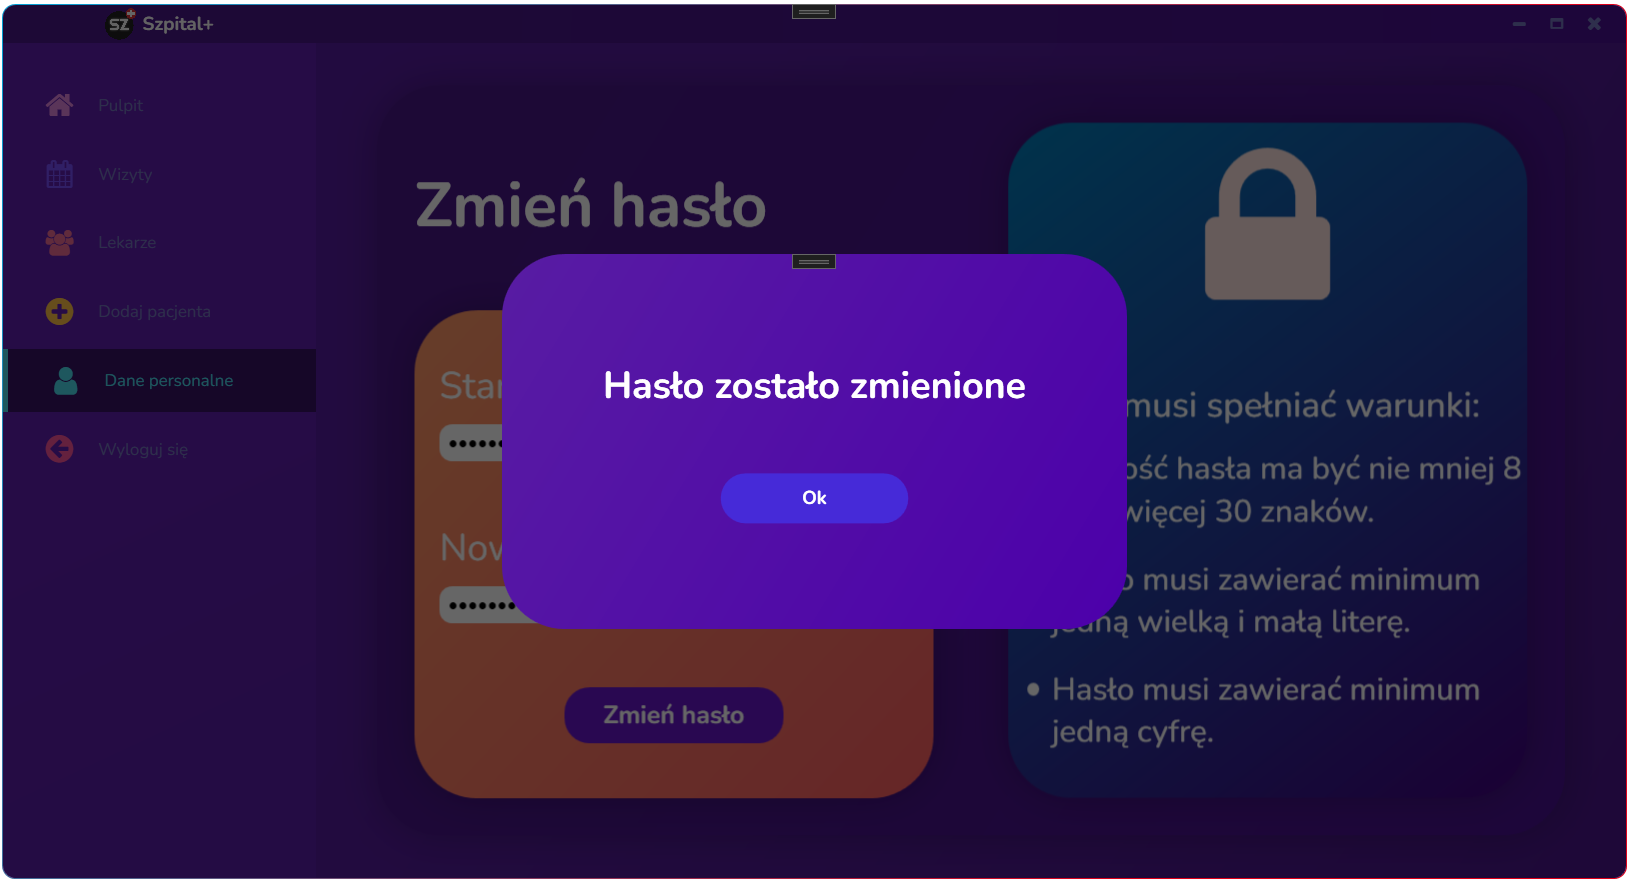
\includegraphics[height=8cm]{images/haslo_zos_zmien_katpa.png}
    \caption{Hasło zostało zmienione}
\end{center}
\end{figure}

\begin{figure}[H]
    \centering
    \subfigure{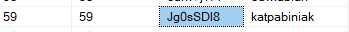
\includegraphics[width=0.4\textwidth]{images/stare_haslo_katpa.png}} 
    \subfigure{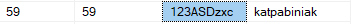
\includegraphics[width=0.4\textwidth]{images/nowe_haslo_katpa.png}}
    \caption{Stare i zmienione hasło}
\end{figure}

\newpage

\section{Okna dla recepcjonisty}
\Large\textbf{{Lekarze}}

\begin{figure}[H]
\begin{center}
    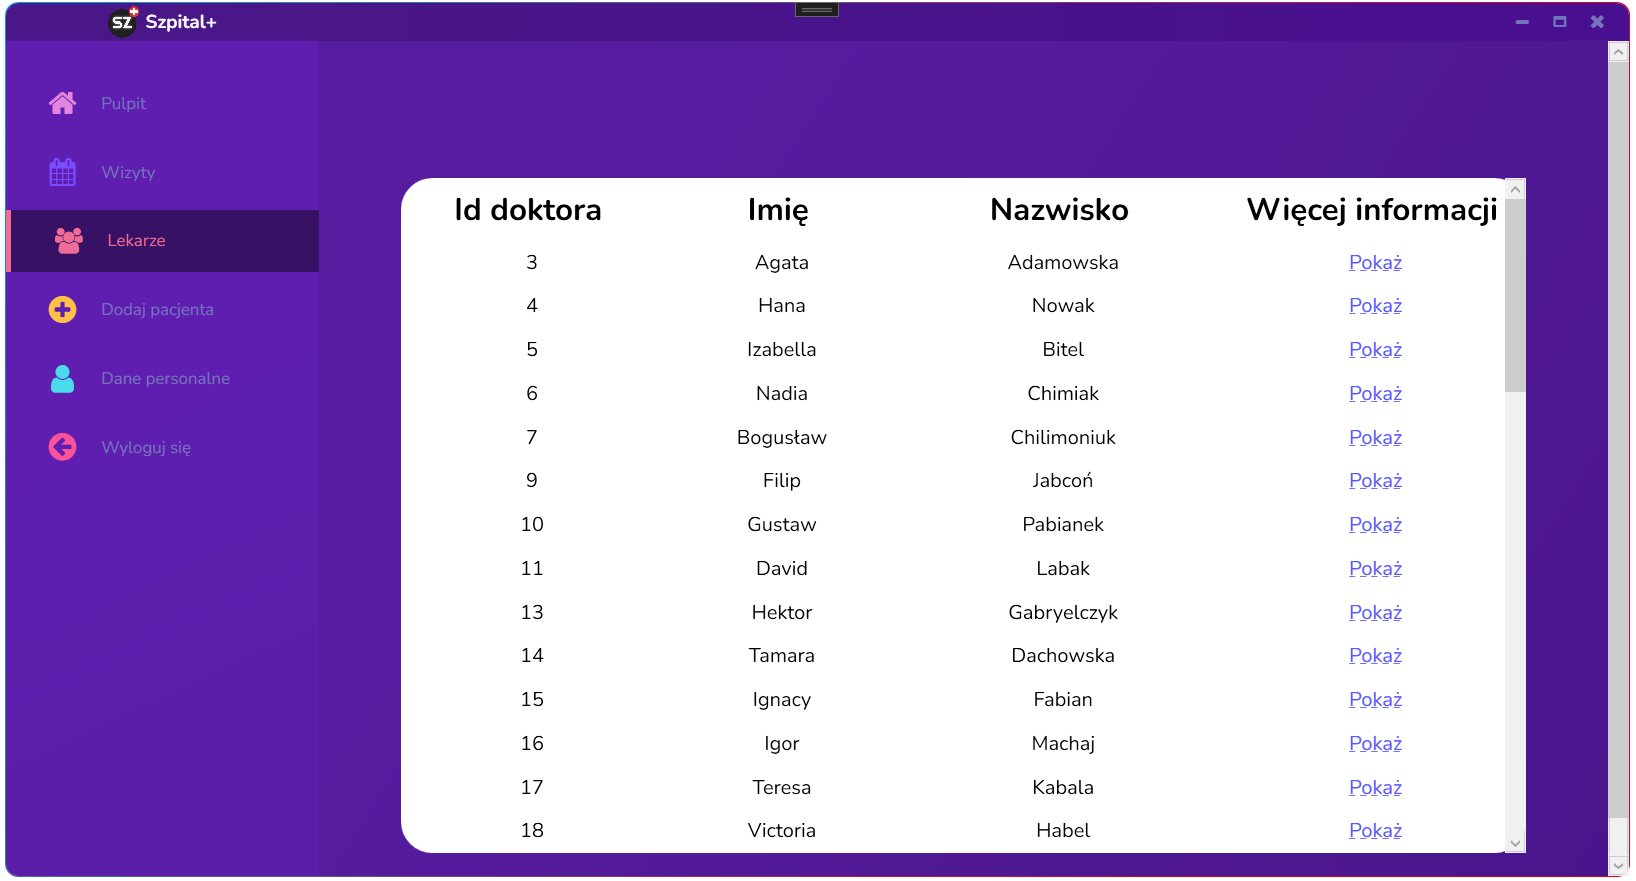
\includegraphics[height=7cm]{images/recep_lekarze.png}
    \caption{Okno recepcjonisty(Lekarze)}
\end{center}
\end{figure}

\Large\textbf{{Dodaj pacjenta}}

\begin{figure}[H]
\centering
    \subfigure{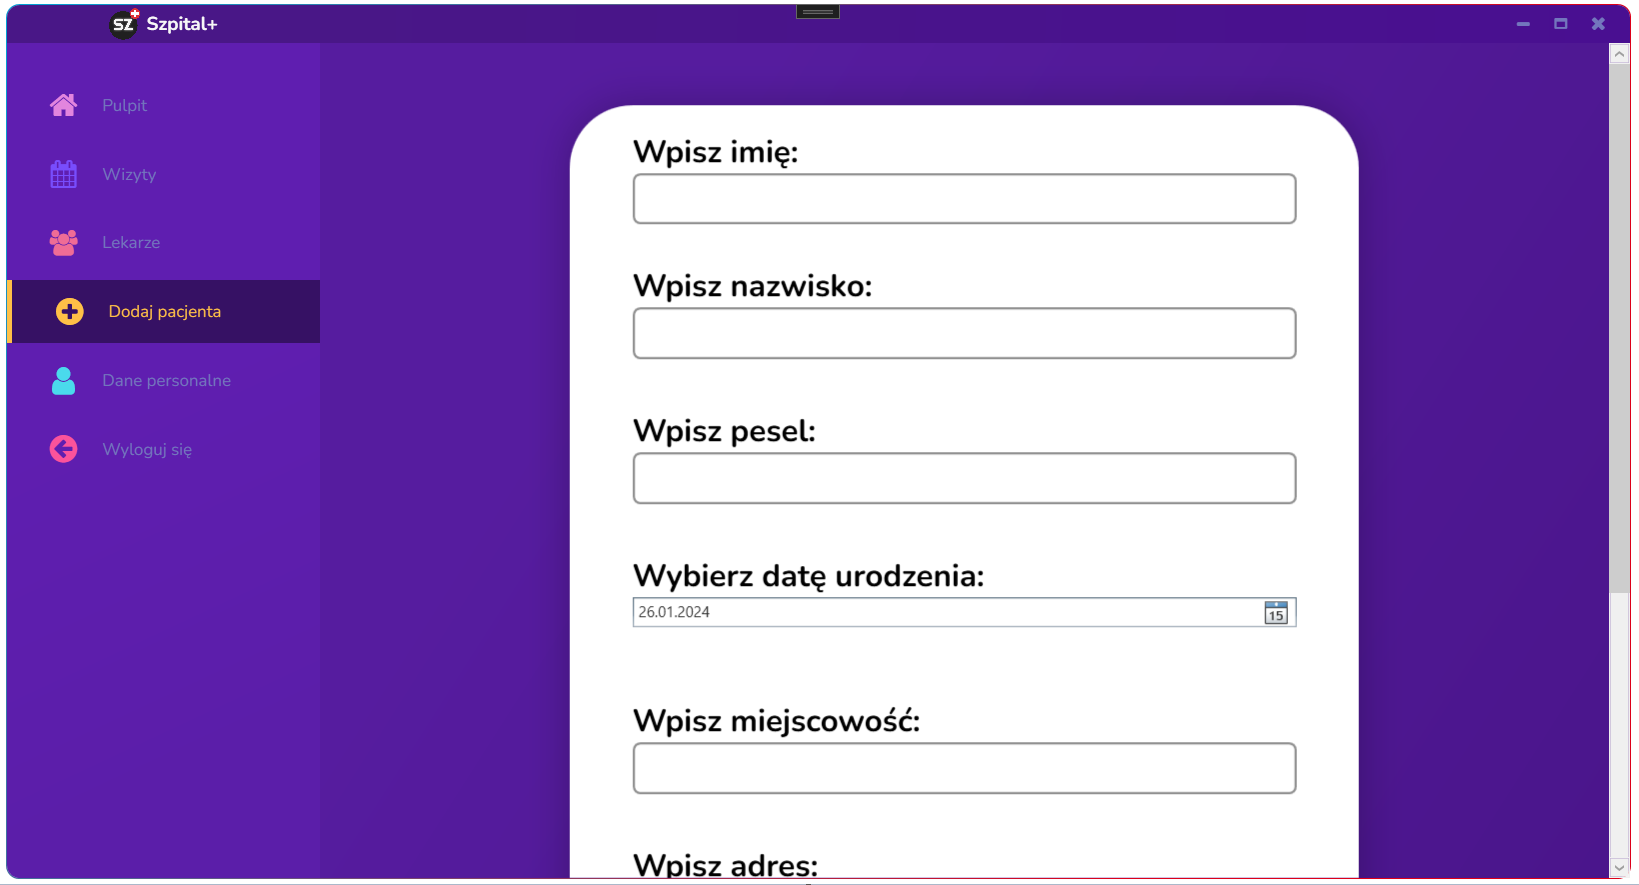
\includegraphics[width=0.6\textwidth]{images/dodaj_pacj_1.png}} 
    \subfigure{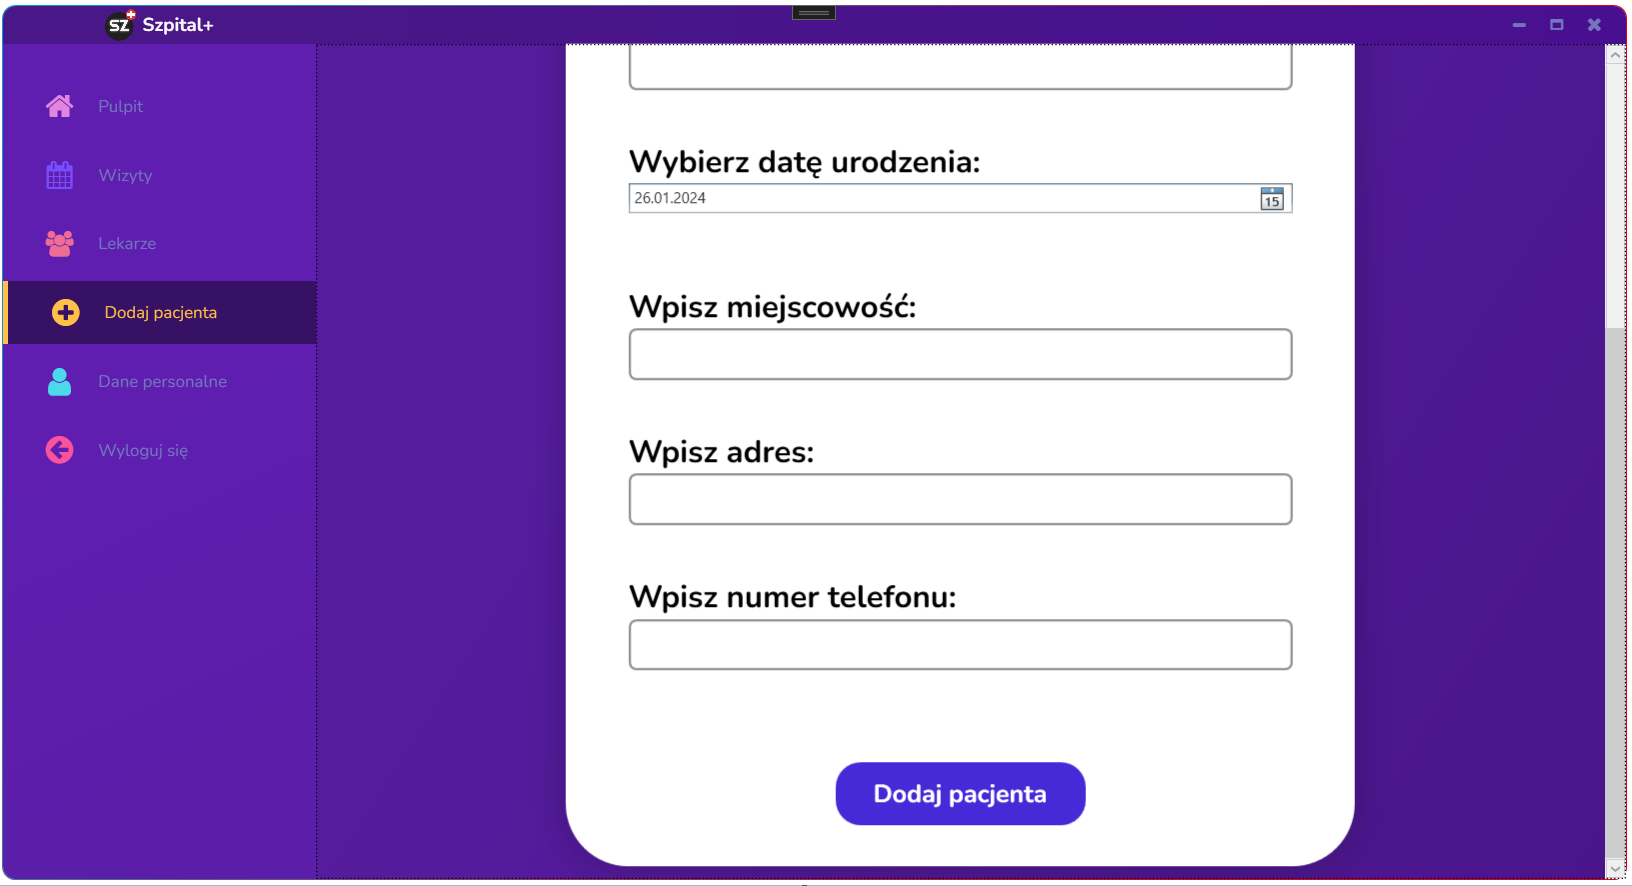
\includegraphics[width=0.6\textwidth]{images/dodaj_pacj_2.png}}
    \caption{Okno recepcjonisty(Dodaj pacjenta)}
\end{figure}

\begin{figure}[H]
    \begin{center}
    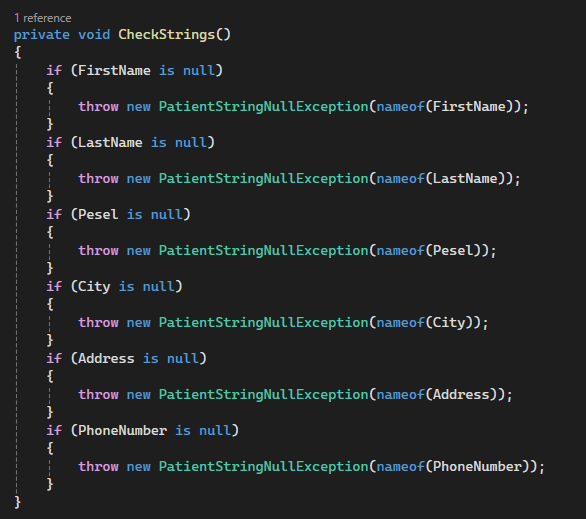
\includegraphics[height=8cm]{images/spraw_null.png}
    \caption{Sprawdzenie na puste pola}
\end{center}
\end{figure}

\begin{figure}[H]
\begin{center}
    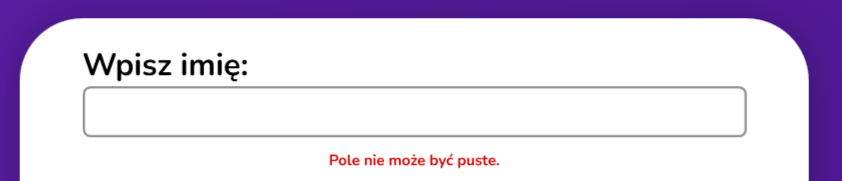
\includegraphics[height=3cm]{images/blad_wpisz_im.png}
    \caption{Wystąpienie błędu przy pustym błędzie}
\end{center}
\end{figure}

\begin{figure}[H]
\begin{center}
    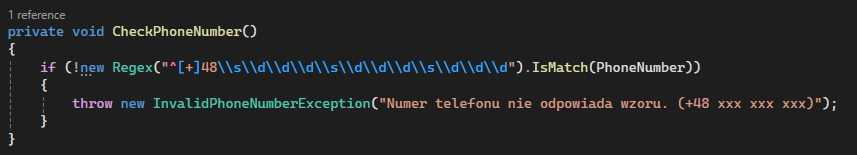
\includegraphics[height=3cm]{images/sprawd_telef.png}
    \caption{Sprawdzenie formatu telefonu}
\end{center}
\end{figure}

\begin{figure}[H]
    \begin{center}
    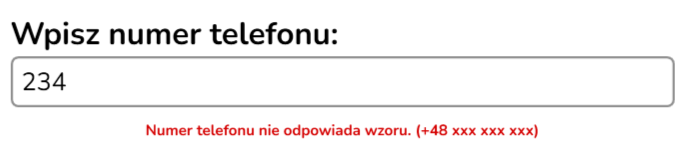
\includegraphics[height=3cm]{images/blad_telef.png}
    \caption{Błąd przy polu numeru telefonu}
\end{center}
\end{figure}

\begin{figure}[H]
\begin{center}
    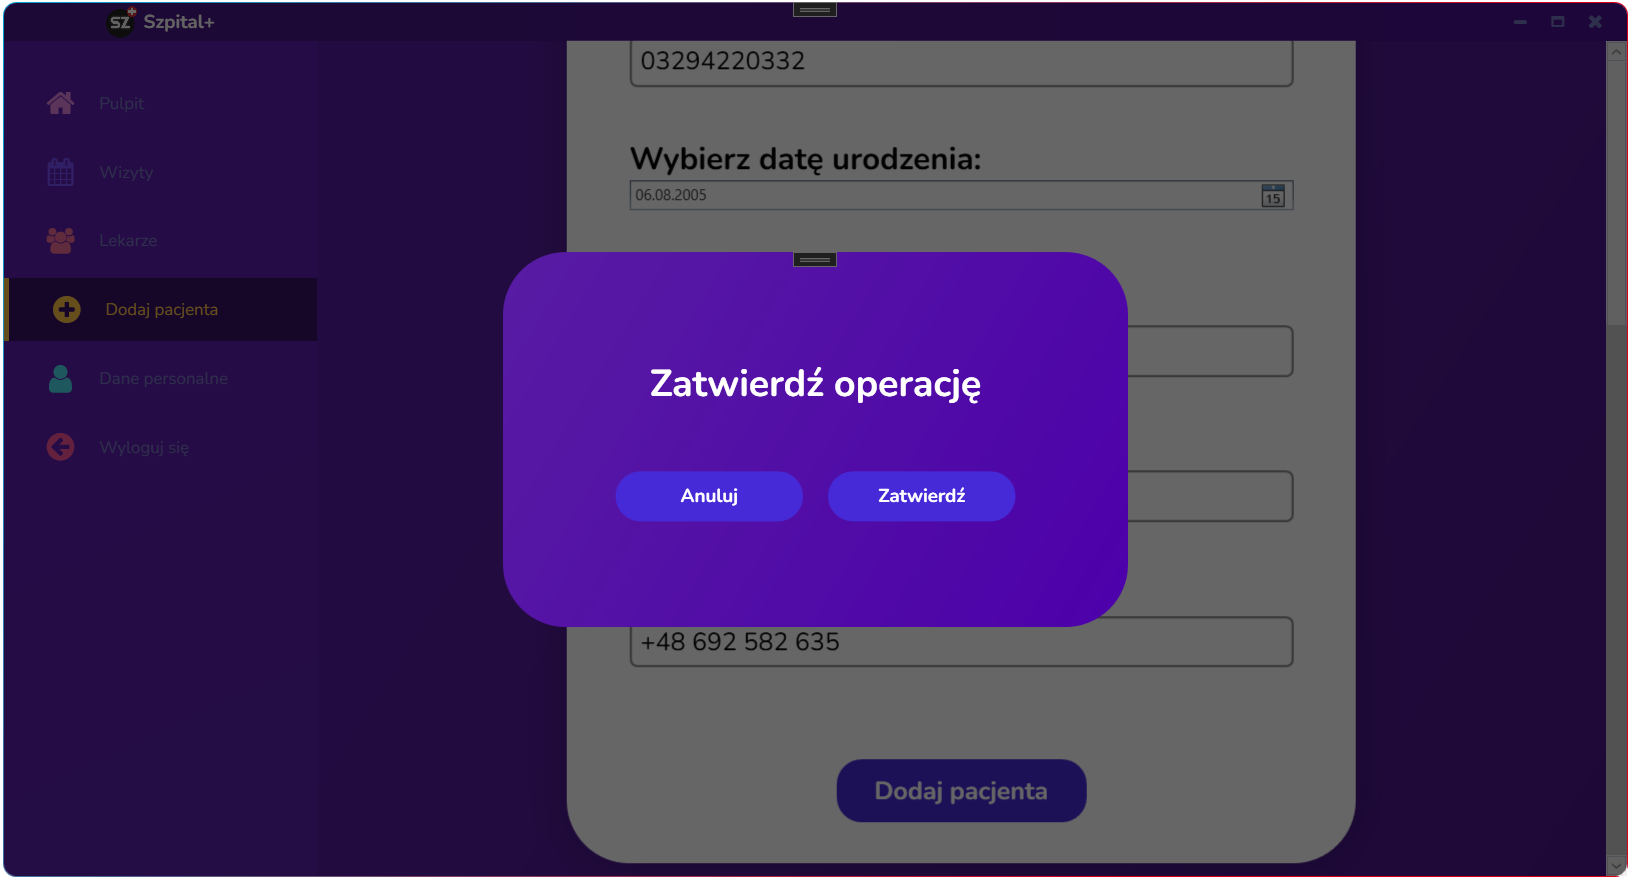
\includegraphics[height=9cm]{images/zatwr_oper_dod.png}
    \caption{Zatwierdzenie operacji}
\end{center}
\end{figure}

\begin{figure}[H]
\begin{center}
    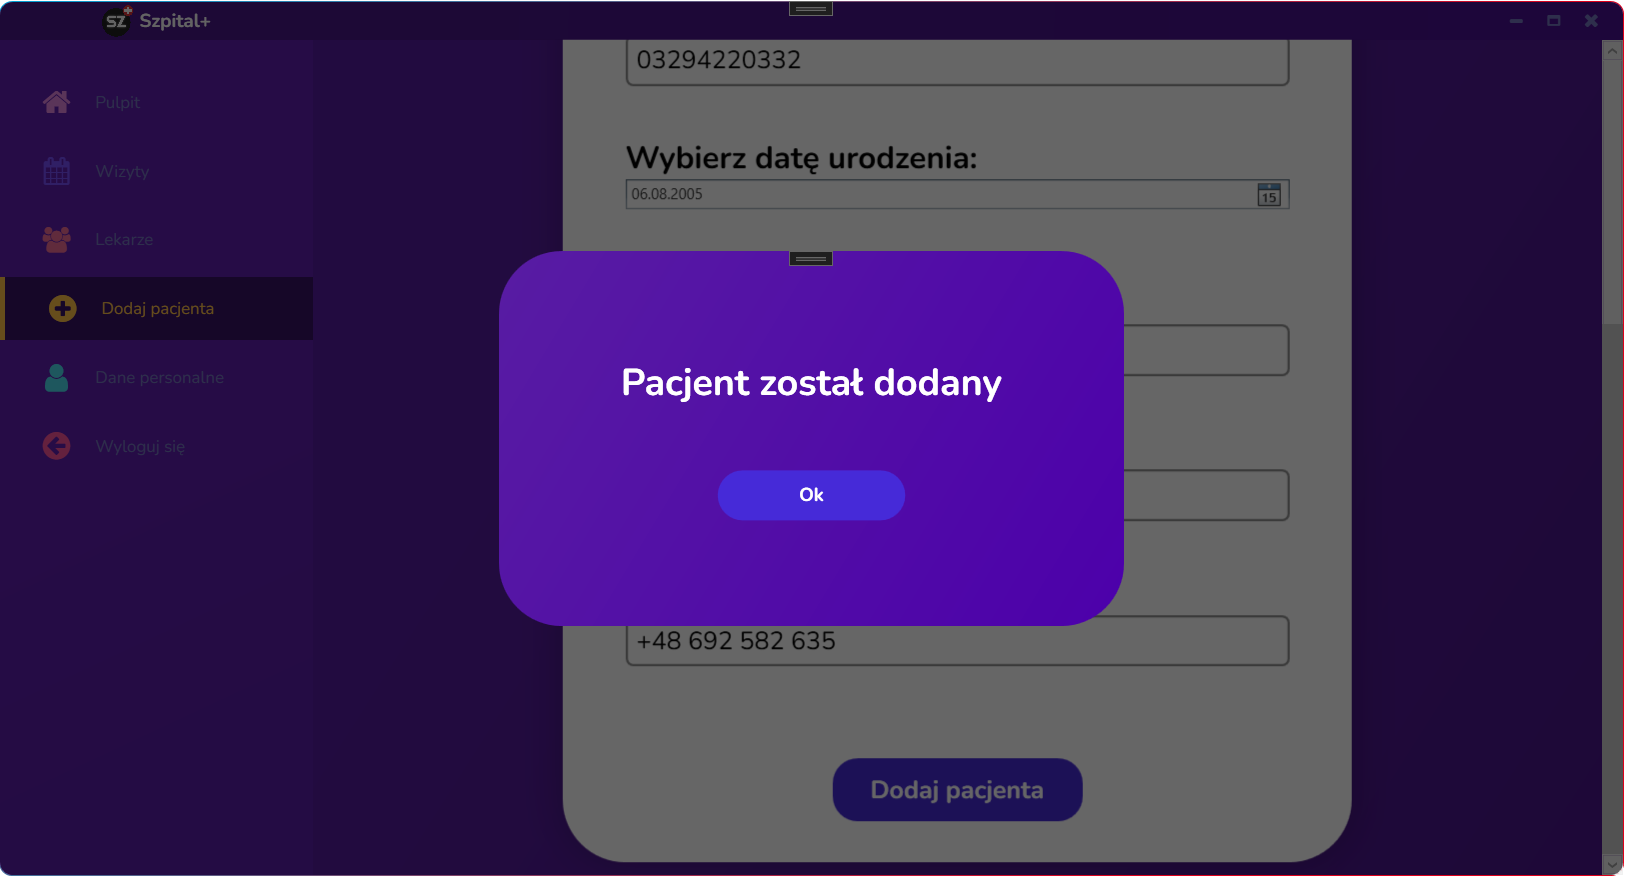
\includegraphics[height=9cm]{images/pacj_zost_dod.png}
    \caption{Pacjent został dodany}
\end{center}
\end{figure}

\begin{figure}[H]
\centering
    \subfigure{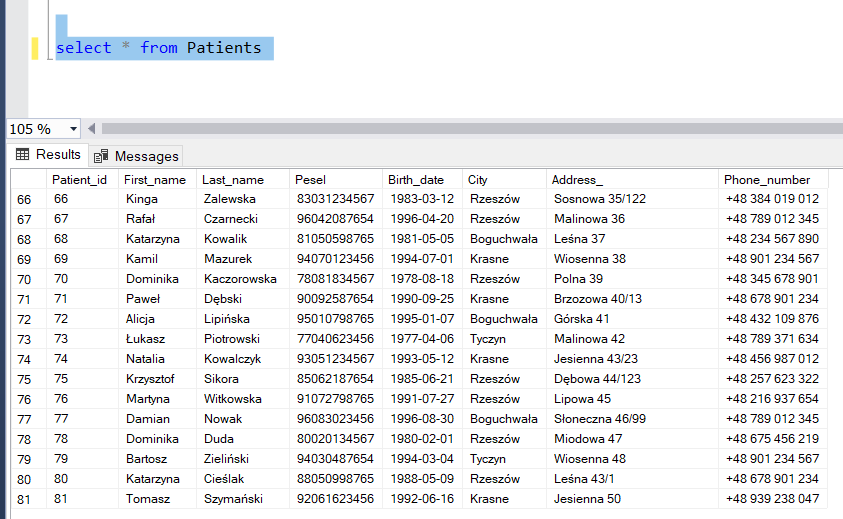
\includegraphics[width=0.6\textwidth]{images/pacjen_przed_dod.png}} 
    \subfigure{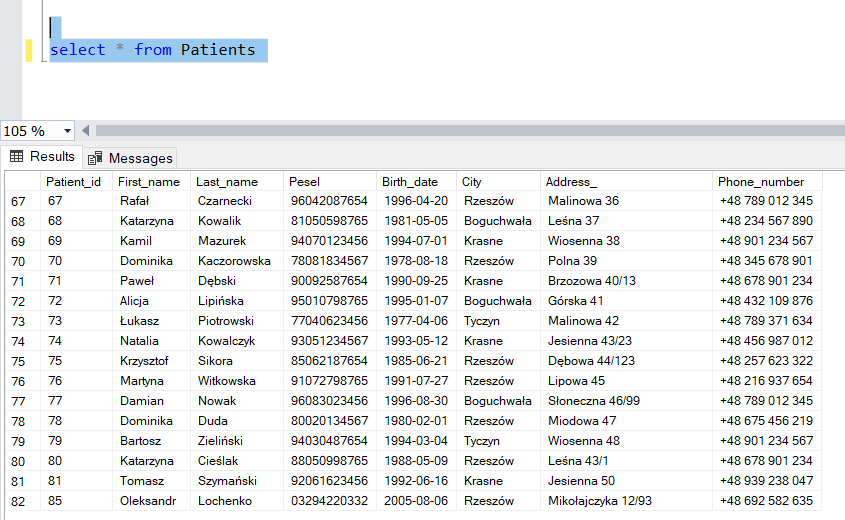
\includegraphics[width=0.6\textwidth]{images/pacjen_po_dod.png}}
    \caption{Tabela pacjentów przed i po dodaniu rekordu}
\end{figure}

\section{Okna dla głównego kierownika}
\Large\textbf{{Pracownicy}}

\begin{figure}[H]
\begin{center}
    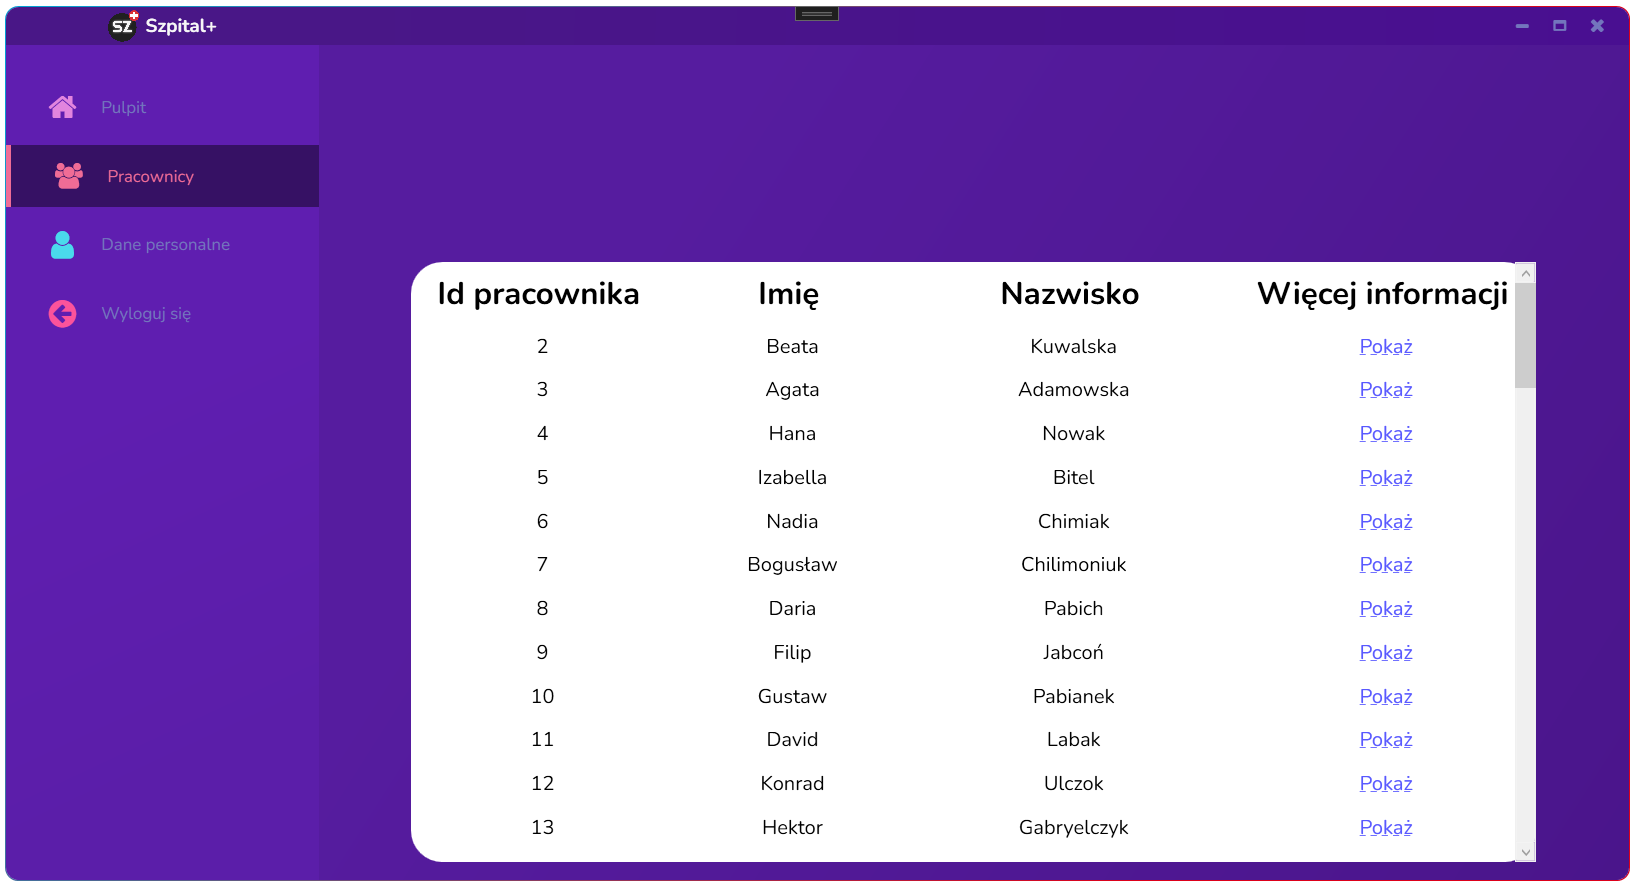
\includegraphics[height=7cm]{images/gl_kier_prac.png}
    \caption{Okno głównego kierownika(Pracownicy)}
\end{center}
\end{figure}

\section{Okna dla kierownika}
\Large\textbf{{Lekarze}}

\begin{figure}[H]
\begin{center}
    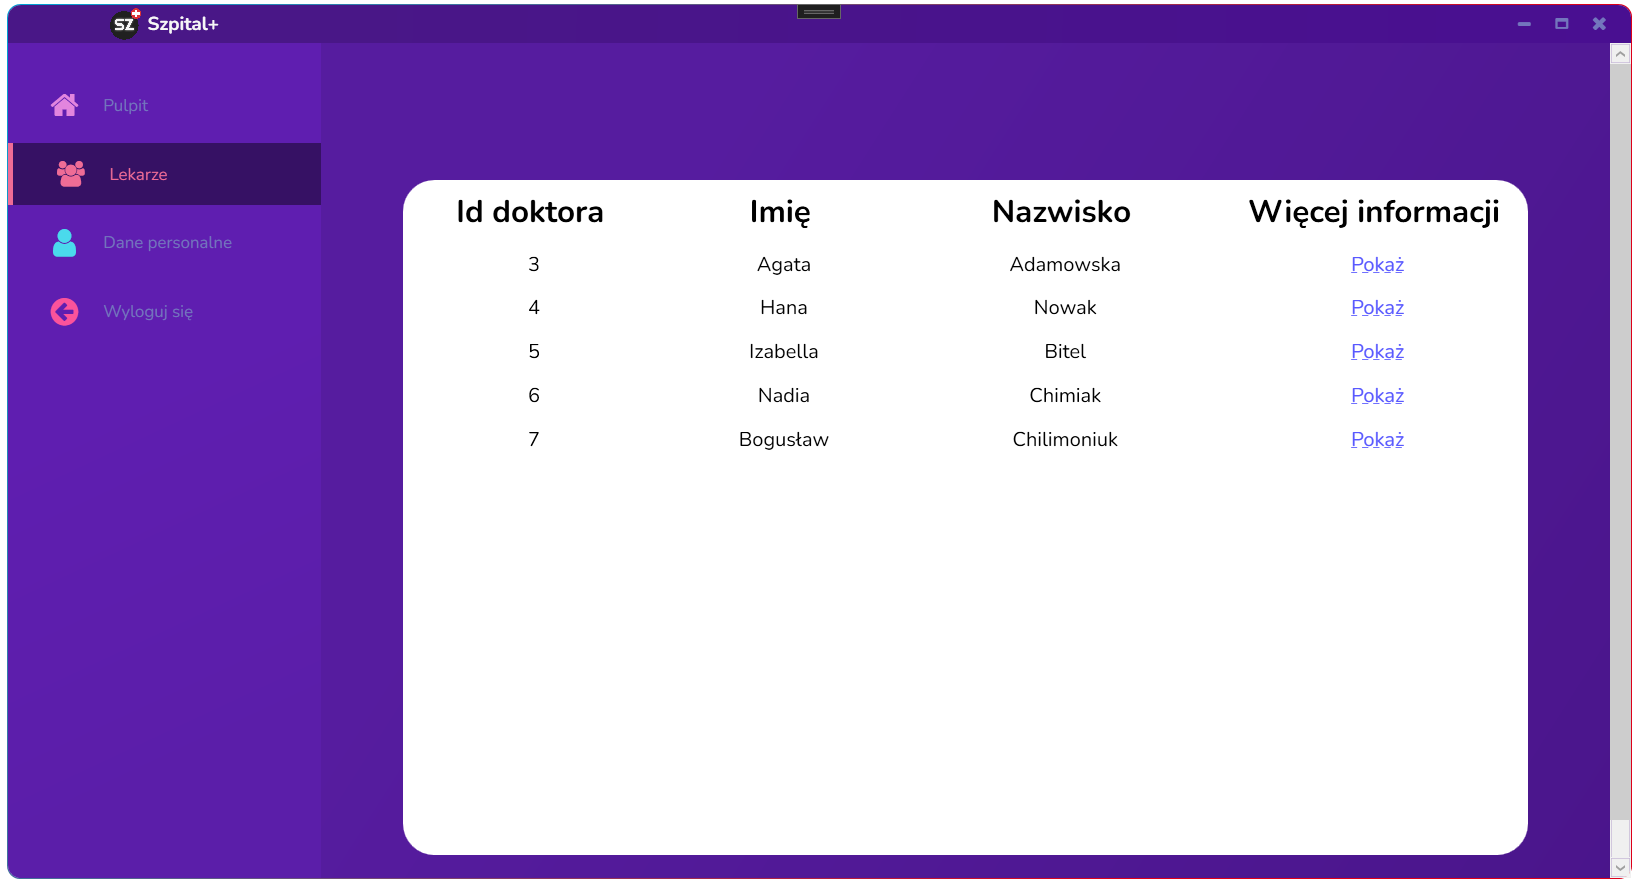
\includegraphics[height=7cm]{images/kier_lekar.png}
    \caption{Okno kierownika(Lekarze)}
\end{center}
\end{figure}

% ********** Koniec rozdziału **********

\newpage
% ********** Rozdział 4 **********
\chapter{Podsumowanie}

Podczas robienia projektu nauczyłem się planowania harmonogramu projektu(\ref{sec:harmon_proj}), implementacji wzoru MVVM(\ref{href:MVVM}), pisania interfejsu użytkownika(\ref{href:XAML}), pracy w środowisku Visual Studio(\ref{href:VStudio}) i programowania w języku C\#(\ref{href:c_sh}).

Dalsza praca będzie polegała na zrealizowaniu wszystkich funkcjonalności których nie zdążyłem zaimplementować, poprawienie i dopasowanie widoków, dodanie animacji oraz ulepszenie wydajności aplikacji.



% ********** Koniec rozdziału **********


\newpage

% *************** Bibliografia ***************
\begin{thebibliography}{6}
\addcontentsline{toc}{chapter}{Bibliografia}
%dodanie wpisu do spisu bibliograficznego

\bibitem{www-1} https://youtu.be/fZxZswmC\_BY?si=gn6SI5tqut9n-vOM
\bibitem{www-2} https://youtu.be/oSeYvMEH7jc?si=aWGmXG\_Enb7S\_z3j
\bibitem{www-3} https://youtu.be/PzP8mw7JUzI?si=twPT-bTfhYE-FMau
\bibitem{www-4}
https://stackoverflow.com/questions/833943/watermark-hint-placeholder-text-in-textbox
\bibitem{www-5}
https://leanactionplan.pl/wykres-gantta/
\bibitem{www-6}
https://pl.wikipedia.org/wiki/Windows\_Presentation\_Foundation
\bibitem{www-7}
https://pl.wikipedia.org/wiki/.NET\_Framework
\bibitem{www-8}
https://pl.wikipedia.org/wiki/Extensible\_Application\_Markup\_Language
\bibitem{www-9}
https://en.wikipedia.org/wiki/Model\%E2\%80\%93view\%E2\%80\%93viewmodel
\bibitem{www-10}
https://stackoverflow.com/questions/58272836/display-datetime-in-textblock-with-dashed-underlined-textdecorations
\bibitem{www-11}
https://stackoverflow.com/questions/30231252/disable-main-window-wpf
\bibitem{www-12}
https://stackoverflow.com/questions/26258450/how-do-i-add-a-bullet-point-in-front-of-a-text-binding-in-wpf
\bibitem{www-13} https://learn.microsoft.com/en-us/archive/msdn-magazine/2009/february/patterns-wpf-apps-with-the-model-view-viewmodel-design-pattern

\bibitem{etykieta1}Rob Miles, {\it C\# Programming Yellow Book}, 2019.
\end{thebibliography}
\newpage

% *************** Zakończenie ***************
% *************** Zakończenie ***************

%***************************************************************************************
% W tym miejscu znajdują się polecenia odpowiedzialne za tworzenie
% spisu ilustracji, spisu treści oraz streszczenia pracy
%***************************************************************************************

%spis rysunków
\addcontentsline{toc}{chapter}{Spis rysunków}
\listoffigures
\newpage

% %streszczenie
% \addcontentsline{toc}{chapter}{Streszczenie}
% \noindent
% {\footnotesize{}\textbf{Wyższa Szkoła Informatyki i Zarządzania z siedzibą w Rzeszowie\\
% Kolegium Informatyki Stosowanej}
% \vspace{30pt}

% \begin{center}
% \textbf{Streszczenie pracy dyplomowej inżynierskiej}\\
% \temat
% \end{center}

% \vspace{30pt}
% \noindent
% \textbf{Autor: \autor
% \\Promotor: \promotor
% \\Słowa kluczowe: tutaj umieść słowa kluczowe}
% \vspace{40pt}
% \\Treść streszczenia, czyli kilka zdań dotyczących treści pracy dyplomowej w języku polskim.
% \vspace{80pt}

% \noindent
% \textbf{The University of Information Technology and Management in Rzeszow\\
% Faculty of Applied Information Technology}
% \vspace{30pt}

% \begin{center}
% \textbf{Thesis Summary\\}
% Tytuł pracy w języku angielskim
% \end{center}

% \vspace{30pt}
% \noindent
% \textbf{Author: \autor
% \\Supervisor: \promotor
% \\Key words: tutaj umieść słowa kluczowe}
% \vspace{40pt}
% \\Treść streszczenia, czyli kilka zdań dotyczących treści pracy dyplomowej w języku angielskim - tłumaczenie tekstu z języka polskiego.
% }

% *************** Koniec pliku back.tex ***************


\end{document}
% *************** Koniec pliku szablon.tex ***************
